\documentclass[12pt]{article}

\usepackage[top=0.75in,bottom=0.75in,left=0.75in,right=0.75in]{geometry}
\usepackage{amsmath,amssymb,multirow,graphicx,natbib}
\usepackage{setspace}

% Comments for making sure we touch all the bases for a good paper
\newif\ifcommentsw
\commentswtrue
\newcommand{\comment}[1]{\ifcommentsw  $\blacktriangleright$\ \textbf{#1}\ $\blacktriangleleft$ \fi}
%\commentswfalse   % remove the % to turn off informational comments 


% Notes on the paper for communicating with coauthors
\newif\ifnotesw
\noteswtrue
\newcommand{\notes}[1]{\ifnotesw  $\bullet$\ \textit{ \textbf{#1}}\ $\bullet$ \fi}
%\noteswfalse   % remove the % to turn off notes to coauthors

\parskip=5pt
\parindent=0pt

\newcommand{\br}{\mathbf{r}}
\newcommand{\sgn}{\operatorname{sgn}}
\def\cq{{\emph{Culex quinquefasciatus}}}
%\newcommand{\mycaption}[1]{\caption{{\footnotesize \textsc{#1}}}}
\usepackage[font={small,singlespacing}]{caption}
\newcommand{\mycaption}[1]{\caption{#1}}
\linespread{1.1}

\title{An agent-based model of mosquito-host encounter rates}
\author{
\textbf{Ricardo Cortez}\\
   \small{Mathematics Department}\\
   \small{Tulane University}\\ \and
\textbf{Bree Cummins}\\
   \small{Mathematics Department}\\
   \small{Tulane University}\\ \and
\textbf{Ivo M. Foppa}\\
   \small{Department of Epidemiology}\\
   \small{Tulane University}\\ \and
   \textbf{James M. Hyman}\\
   \small{Mathematics Departmen}\\
   \small{Tulane University}\\ \and
\textbf{Justin Walbeck}\\
   \small{Mathematics Department}\\
   \small{Tulane University}\\ 
}


\begin{document}
	
	\tableofcontents
	
	\maketitle

\abstract{
%
%\comment{\it  {\bf Start with the principal result of the paper}} 
%
We develop and analyze  a hybrid mathematical model to explore the effect of spatial 
heterogeneity on the encounter rate between mosquito vectors and bird hosts.  
%
%\comment{\it  {\bf state the problem being addressed and why it is important}} 
%
The mosquito host-seeking behavior and heterogeneity in the distribution of hosts are important factors in predicting the transmission 
dynamics of mosquito-borne infections  such as the spread of the West Nile virus.   Ignoring heterogeneity in transmission models can result in misleading insights into the transmission dynamics.  
%
%\comment{\it  {\bf what has been done and the bottleneck that has kept the problem from being solved}} 
% 
%
% \comment{\it  {\bf The objective of this research and how it will advances the solution of the problem}} 
%
Host-seeking mosquitoes use different host seeking strategies in guiding them to a blood meal.  When odor plumes and not present, the mosquitoes engage in ranging flight behavior, influenced by the wind velocity.  When they pick up the scent of a host, then their flight is influenced by both the wind velocity and odor cues.
%
%\comment{\it  {\bf State the principle results}}
% 
Our model includes behavioral rules for the 
flight of discrete host-seeking mosquitoes, a continuum model for the spreading odor plume 
generated by resting hosts, and stochastic non-uniform wind conditions. 
We model several strategies for using the odor plume  in different 
wind conditions to locate a host and quantify their relative effectiveness. 
We use sensitivity analysis to determine that the model predictions are most sensitive to  ******* .  
%
%\comment{\it  {\bf How these results advance the understanding of the problem}} 
%  
We find that our hybrid model is an effective approach to simulate mosquito host-seeking behavior and that mosquitoes could use either the local odor concentration or the odor gradient to guide their flight. 
}

\textbf{Keywords} Mosquito $\cdot$ Mathematical Model $\cdot$ West Nile virus  $\cdot$ odor plume
	
%%%%%%%%%%%%%%%%%%%
\section{Introduction}
%%%%%%%%%%%%%%%%%%%
\comment{\it  {\bf Make it clear to the reader what the main idea of the paper is after the first 3-5 paragraphs of the introduction and give a clear picture of what is to come in the paper.   }}

We develop and analyze a mathematical model to simulate the host-seeking behavior of mosquitoes that can be applied to the transmission of mosquito-borne diseases.  The mosquitoes are modeled as discrete { \em agents} that fly in a continuum model for the wind seeking discrete hosts (birds).  The flight direction and speed of individual mosquitoes is influenced by both the wind and odors emitted by the host. 
We use the model to compare the effectiveness of different flight strategies in finding the host and quantify the sensitivity our our results to our assumptions for the model parameters.   We find that the there are a broad range of effective host-seeking strategies that are insensitive out detailed assumptions of the parameter values. 

Transmission of many infectious agents is heterogenous in the sense that the risk for infection and infectiousness are unevenly distributed over the population~\cite{Woolhouse1997}. This heterogeneity is an important factor in predicting the spread of an infection and ignoring heterogeneity in transmission models can result in misleading inference about transmission dynamics.  The heterogeneity is particularly important with the infection is at very levels, such as the prevalence of Wet Nile virus (WNV), and mathematical models that do not account for the heterogeneity can underestimate the probability that infectious agent will persist ~\cite{Hasibeder1988}.
One source of heterogeneity in mosquito--borne disease transmission is the nonuniform distribution of mosquito 
bites over hosts~\cite{Dye1986}, which depends on  the number of mosquitoes that find that host.
Host finding of mosquitoes is largely driven by olfactory cues that are given off by individual hosts~\cite{Lehane1991}.
We might therefore expect that  the way feeding hosts of mosquitoes are spatially arranged will affect the mosquitoes' probability of success in locating and feeding on them. Most vertebrate hosts are spatially aggregated.
Unless the probability of finding a host is exactly proportional to the local density of hosts,
unevenly distributed biting rates on individual hosts and thus heterogenous disease transmission will result.

This is an important observation for the American crow (\textit{Corvus brachyrhynchos}) and other species of 
birds that are particularly vulnerable to WNV infection and tend to congregate in large roosts.  An 
immediate question is {\em How does the roosting behavior of birds and catastrophic changes in roost structure 
affect the transmission dynamics of this mosquito--borne virus?} 
Answering this question motivates the work presented here. It requires a detailed understanding of how the spatial arrangement of hosts will affect the distribution of mosquito bites on these hosts.
%
The difficulties in approaching this question experimentally makes agent-based simulations a natural way 
to explore this problem under a range of assumptions about host distribution, mosquito behavior, and odor dispersal.

We will use mathematical modeling to address the effect of host aggregation on a small-scale spatial on the per--capita 
biting rate.   Specifically, we present a model for the simulation of host-seeking behavior of mosquitoes that 
applies to the transmission of West Nile Virus or other mosquito-borne diseases.  The model accounts for
host-seeking behavior in both ranging flight, influenced by wind velocity, and homing flight, guided by both wind velocity and odor cues.  There is little experimental data for the parameters in a host-seeking mosquito model.  We use sensitivity analysis to quantify the uncertainty in our predictions as a function of changes in our assumptions.   The sensitive analysis shows that the ability of mosquitoes to find a host is relatively insensitive to our model assumptions. 

We analyze  the difference between host-seeking models based on the local concentration of the odor plume and and models based on the gradient of the odor plume.   We find that under some conditions, these different approaches are both effective and do not show statistically significant differences in a mosquito's ability to locate a host.  

\comment{\it  {\bf After the introduction, the reader should understand the importance of this problem and what contribution the authors made to solving a problem. }}

%%%%%%%%%%%%%%%%%%%%%
\section{Mosquito host-seeking behavior}\label{sec:mosqbehav}
%%%%%%%%%%%%%%%%%%%%%%
The diurnal cycle triggers host-seeking behavior in mated female mosquitoes. Typically this behavior begins when the mosquitoes are far from the hosts and ends after a successful bite.  Our model assumes that the mosquito host-seeking behavior takes place between tens of meters and tens of centimeters from a host. On this scale, it is useful to classify the host-seeking behavior in terms of two functional regimes that we will call  {\em homing flight} (flight influenced by the presence of an odor cue) and { \em ranging flight} (flight without an odor cue).  

%%%%%%%%%%%%%%%%%%%%%%
\subsection{Homing flight}
%%%%%%%%%%%%%%%%%%%%%%
When a mosquito detects an odor plume from a host, it uses the odor plume and the wind to guide its homing flight to locate the host.
Odor cues are complex olfactory signals released from a host's skin and breath. There are many chemicals known to excite the chemoreceptors of mosquitoes, for example CO$_2$, lactic acid, and various 
aldehydes~\cite{Bowen1991,Syed2009}. CO$_2$ is a very important component in the odor plume that activates and helps maintain homing flight~\cite{Bowen1991,Gibson1999,Gillies1980}. It has been reported that activation thresholds for the mosquitoes \emph{Aedes aegypti} and \emph{Anopheles gambiae} are 100-300 ppm (0.01-0.03\%)~\cite{Gibson1999} and that mosquitoes are sensitive to changes in CO$_2$ concentration as small as 100 ppm~\cite{Gillies1980}.

Odor plume structure is important to mosquito behavior. Laboratory wind tunnel experiments indicate that
sustained flight only occurs in the presence of an intermittent CO$_2$ signal and not in uniform 
concentrations~\cite{Gillies1980}.  In~\cite{Dekker2005,Dekker2001} it is reported that broad, 
well-mixed CO$_2$ plumes inhibit upwind flight while turbulent plumes of the same concentration induce 
upwind flight in a laboratory wind tunnel.

Wind also plays a role in the way odor cues are spread.  In the absence of wind, chemical signals are dispersed primarily by diffusion. In the presence of uniform, laminar wind, the host odor extends into a long, thin plume with sharp transverse gradients and shallow longitudinal gradients. If the wind is turbulent, then the plume is characterized by a high degree of intermittency, but it still retains relatively shallow average longitudinal gradients compared to the transverse 
gradients~\cite{Vickers2000}. 

Mosquitoes must be able to locate hosts both in windy and windless conditions. In the absence of wind, mosquitoes must rely solely on odorant cues \cite{Vickers2000} or on large features in the visual environment~\cite{Bidlingmayer1994}. If an odorant signal is present, mosquitoes may sample the odorant over time to estimate the gradient, as is conjectured for tsetse flies~\cite{Carde1996}. 
%
When there is wind present as well as an odorant cue, laboratory and field wind tunnel experiments~\cite{Cooperband2006, Dekker2005,Dekker2001} indicate that mosquitoes travel upwind to locate the source. They estimate the wind direction by watching the optical flow of ground features \cite{Carde1996}. Wind speeds of interest are low, since a typical flight speed for mosquitoes 1 m/s or less~\cite{Clements1999}. 
 It is known that many organisms have characteristic turns in their upwind flight path (e.g. moths~\cite{Carde1996,Vickers2000}), but mosquitoes and tsetse flies exhibit highly irregular upwind flight~\cite{Davis1996}.

%%%%%%%%%%%%%%%%%%%%%%
\subsection{Ranging flight}
%%%%%%%%%%%%%%%%%%%%%%
In the absence of odor cues, mosquitoes use ranging flight, influenced by wind currents, to locate odor plumes.  Unlike homing flight, ranging flight behavior remains mostly uncharacterized. If wind is absent, orientation may be determined by large visual features in the 
environment~\cite{Bidlingmayer1994} or may be characterized as an unbiased random walk. If wind is present, then the mosquitoes may deliberately choose to fly upwind, downwind, or crosswind in search of a host. Each of these three behaviors has been described as plausible based on either experimental or theoretical work. 
Mosquitoes typically fly upwind in wind tunnels even when there is no odorant present~\cite{Gibson1999}. 
A set of field experiments reported in~\cite{Gillies1974} provided evidence for downwind flights in host-seeking
 \emph{Mansonia} mosquitoes. 
In~\cite{Dusenbery1989} it is argued that crosswind searching is mathematically optimal when the odor plumes are long and thin.  If the variability of the wind direction is greater than 30 degrees, either upwind or downwind searching is mathematically optimal~\cite{Sabelis1984}.



%%%%%%%%%%%%%%%%%%%%%%
\section{Model Formulation}
%%%%%%%%%%%%%%%%%%%%%%
 \comment{\it{\bf Describe how the model was developed to answer the research question. 
 Give full details of the chosen methodology so that an interested reader could repeat it. 
Follow a logical order, usually from simple to more complex, or chronological.
A graphic image, which visualizes the model, can be an effective and important attention-grabber. Don't hesitate to use extended figure captions that fully describe the figure (including defining the the axes of all graphs).  Be sure to point out explicitly what you want to reader to see in each figure.  Don't assume that the reader will see what you think is obvious.  Use an adequate font size in the figure and be sure that the text on your figures does not require a magnifying glass to read.
}}


We model the mosquitoes and hosts as individuals, or agents.  The hosts emit a CO$_2$ odor plume that is carried by the wind and stochastic diffusion in the air.  The CO$_2$ distribution modeled by an advection-diffusion partial differential equation.  We use a biased random walk to model the mosquitoes flying and seeking the hosts. 
The mosquito flight is restricted to  a two-dimensional rectangular region whose sides are of length $L_x$ and $L_y$. A population of $N_v$ mosquitoes (e.g. {\sl Cx. quinquefasciatus}) are given independent entrance times and entrance locations into the domain. Initial populations of $N_h$ hosts (e.g. birds) are placed in several subregions of the domain.

The model is formulated in terms of how the mosquitoes seek out their hosts by locating and following an odor plum.   We construct a modeling framework that can accommodate different ranging and host-seeking mosquito behavior, wind velocities, locations of the hosts, and other physical and biological scenarios. 

%%%%%%%%%%%%%%%%%%%%%%	
\subsection{Odor plumes}
%%%%%%%%%%%%%%%%%%%%%%
The hosts release a fixed amount of CO$_2$ (or some other gaseous cues) per host per
unit time.  This concentration plume is diffused and convected by wind within a
two-dimensional region. The convection velocity of the wind is given by
a velocity vector ${\vec V}(x,y,t)$.  The concentration $C(x,y,t)$ of CO$_2$ is transported and 
diffused by the  equation
\begin{equation}\label{eq:conv-diff}
\frac{\partial C}{\partial t} + \nabla\cdot ( {\vec V} C ) = D\nabla^2 C + C_s(x,y),
\end{equation}
\[
\mbox{with } \vec{V}(x,y,t) = \vec{U}(x,y,t) + \vec{U_r}(x,y,t)
\]
where $t$ is time, and $(x,y)$ are spatial coordinates.  The constant diffusion coefficient $D$ is adjusted to reflect the speed at which the particular substance of interest diffuses in air.
The transport velocity $\vec{V}$ consists of two components: $\vec{U}$ is used to introduced drifts or 
relatively large features produced by the air; $\vec{U}_r$ is a random velocity vector with mean zero
introduced to approximate the effect of small-scale wind variations in the domain.  The last term
in Eq.~(\ref{eq:conv-diff}) represents the source of CO$_2$ concentration at the host locations. 
In our model, we will consider this term to be 
$C_s(x,y) = J_0 \int\!\!\!\int \delta(x-x_h-z_1,y-y_h-z_2) dz_1 dz_2$ where $J_0$ is a constant 
concentration emission per unit time and the delta function reflects the fact that the CO$_2$ 
occurs only at the host locations $(x_h,y_h)$.
		
To simulate the evolution of the CO$_2$ concentration, we use a discrete grid of spacing $h$ that covers the two-dimensional
domain $\Omega = [0,L_x] \times [0,L_y]$.  We define $h = L_x/N_x = L_y/N_y$ and the cell centers
$x_j = (j-1/2)h$ for $j = 1, 2, \cdots, N_x$.  Similarly, $y_k= (k-1/2)h$ for $k = 1, 2, \cdots, N_y$.
Then $C^n_{j,k}$ approximates $C(x_j,y_k,t_n)$.  We use second-order centered differences to approximate the Laplacian and we use a first-order conservative upwind scheme for the advection terms. We assume that the normal components of the concentration gradient are zero at the boundary (Neumann conditions). The CO$_2$ concentration is updated in discrete time steps of $\Delta t$ using Euler's method.

%%%%%%%%%%%%%%%%%%%
\subsection{Mosquito Behavior}
%%%%%%%%%%%%%%%%%%%
Motivated by the encounter rate between birds and \cq, which is a nocturnal species, the principal opportunities for host-mosquito interaction are during roosting periods in which the birds are relatively stationary. For this reason, the agents representing bird hosts do not move from their initial positions; however, a random walk or biased random walk could be easily introduced.  Mosquitoes, on the other hand, 
will move by taking steps from a random walk where each step direction and length are selected from 
a behavioral rule set. The host and mosquito locations are not restricted to the CO$_2$ grid.

%%%%%%%%%%%%%%%%%%%%%%
%\subsubsection{Mosquito behavioral rules based on CO$_2$ concentration and wind velocity}\label{sec:rules}
%%%%%%%%%%%%%%%%%%%%%%%
Our model accounts for two distinct mosquito behavioral regimes: ranging flight that occurs before a CO$_2$ signal is detected, and homing flight that occurs in the presence of CO$_2$.  It also accounts for the possible loss of the
CO$_2$ signal.  In general, each step of a mosquito is defined by a direction and a speed. A {\em target} direction $\theta$ and a corresponding interval of angles 
$[\theta-\alpha, \theta+\alpha]$ centered around the target direction are computed based on the wind
direction and CO$_2$ concentration (see below).  The step is then taken in a direction chosen from a uniform 
distribution in the interval.
%
The speed of the step is bounded between a maximum and a minimum imposed speed and is found through a deterministic function of concentration and wind speed. A detailed description is given below.

{\bf Model assumptions:}
\begin{itemize}
\item
Below a CO$_2$ threshold $C < C_0$, the mosquitoes navigate only using wind direction and move upwind, downwind, or crosswind.
\item
Above the threshold, the mosquitoes respond to concentrations by moving both upwind 
and up-gradient using CO$_2$ cues. There are saturation levels $C_{sat}$ and $G_{sat}$ above which no further
changes in concentration or gradient can be detected.
\item
Large concentrations (or large concentration gradients) lead to a narrower window from which a mosquito
chooses its direction.  Lower concentrations are considered to be less accurate information and therefore
produce a larger interval around the target direction.
\item
Since mosquito motion is not restricted to the CO$_2$ grid, the mosquitoes may leave and re-enter the 
concentration domain. 
\item
When a mosquito comes within a predetermined radius of a host, the mosquito is removed from the simulation 
and a ``contact" is recorded. In this context, a contact means an attempted landing or bite, not necessarily successful. 
\end{itemize}
	
	
\subsubsection{Concentration gradients}  
Consider a model based on concentration gradient.  The CO$_2$ 
gradient is computed on the grid using finite differences and then it is interpolated to the mosquito location.
The direction $\theta$ of the gradient is the target direction for the mosquito's next step.  Given that there is inaccuracy
in the ability for a mosquito to determine this direction, we produce a window of directions from which the
mosquito will choose randomly.  The size of the window varies inversely to the magnitude of the concentration
gradient as follows.

Let $G_{sat}$ be the maximum concentration gradient that can be sensed and define the 
normalized gradient at  the mosquito location by $b = |\nabla C|/G_{sat}$.  Let the threshold 
concentration gradient be a proportion of the saturation gradient $G_0 = b_0\ G_{sat}$ and 
let $\kappa$ be any number in the range
$(-1/b_0,\infty)$.  The window $[\theta-\alpha,\theta+\alpha]$ (see Fig.~\ref{MosquitoGradient}) is computed from
\begin{equation} \label{eqn:response}
\alpha = \alpha_{max} - (\alpha_{max}-\alpha_{min}) F(b,b_0;\kappa)
\end{equation}
where $\alpha_{max}$ and $\alpha_{min}$ are free parameters and the transition function is set to
\begin{equation}
F(b, b_0; \kappa) = \left\{ \begin{array}{lr} 
   0, & b < b_0 \\ 
   \dfrac{(1+\kappa b_0)(b-b_0)}{(1+\kappa b_0 b)(1 - b_0)}, & b_0 \leq b \leq 1 \\ 
   1, & 1 < b  
   \end{array}\right. . \label{eqn:functional}
 \end{equation}
This ensures that the interval size $\alpha$ takes on the highest values when the sensory input is lowest. The parameter $\kappa$ controls the concavity of the transition function as shown in Figure~\ref{fig:exampleF}.
Once the window of possible step directions is found, the mosquito takes a step in a direction given by a 
random variable uniformly distributed in the window interval:
\begin{equation*}
	\theta_c \in [\theta-\alpha,\theta+\alpha]. %\label{eqn:cdirchoice}
\end{equation*}


\begin{figure}[htp]
\begin{tabular}{ccc}
	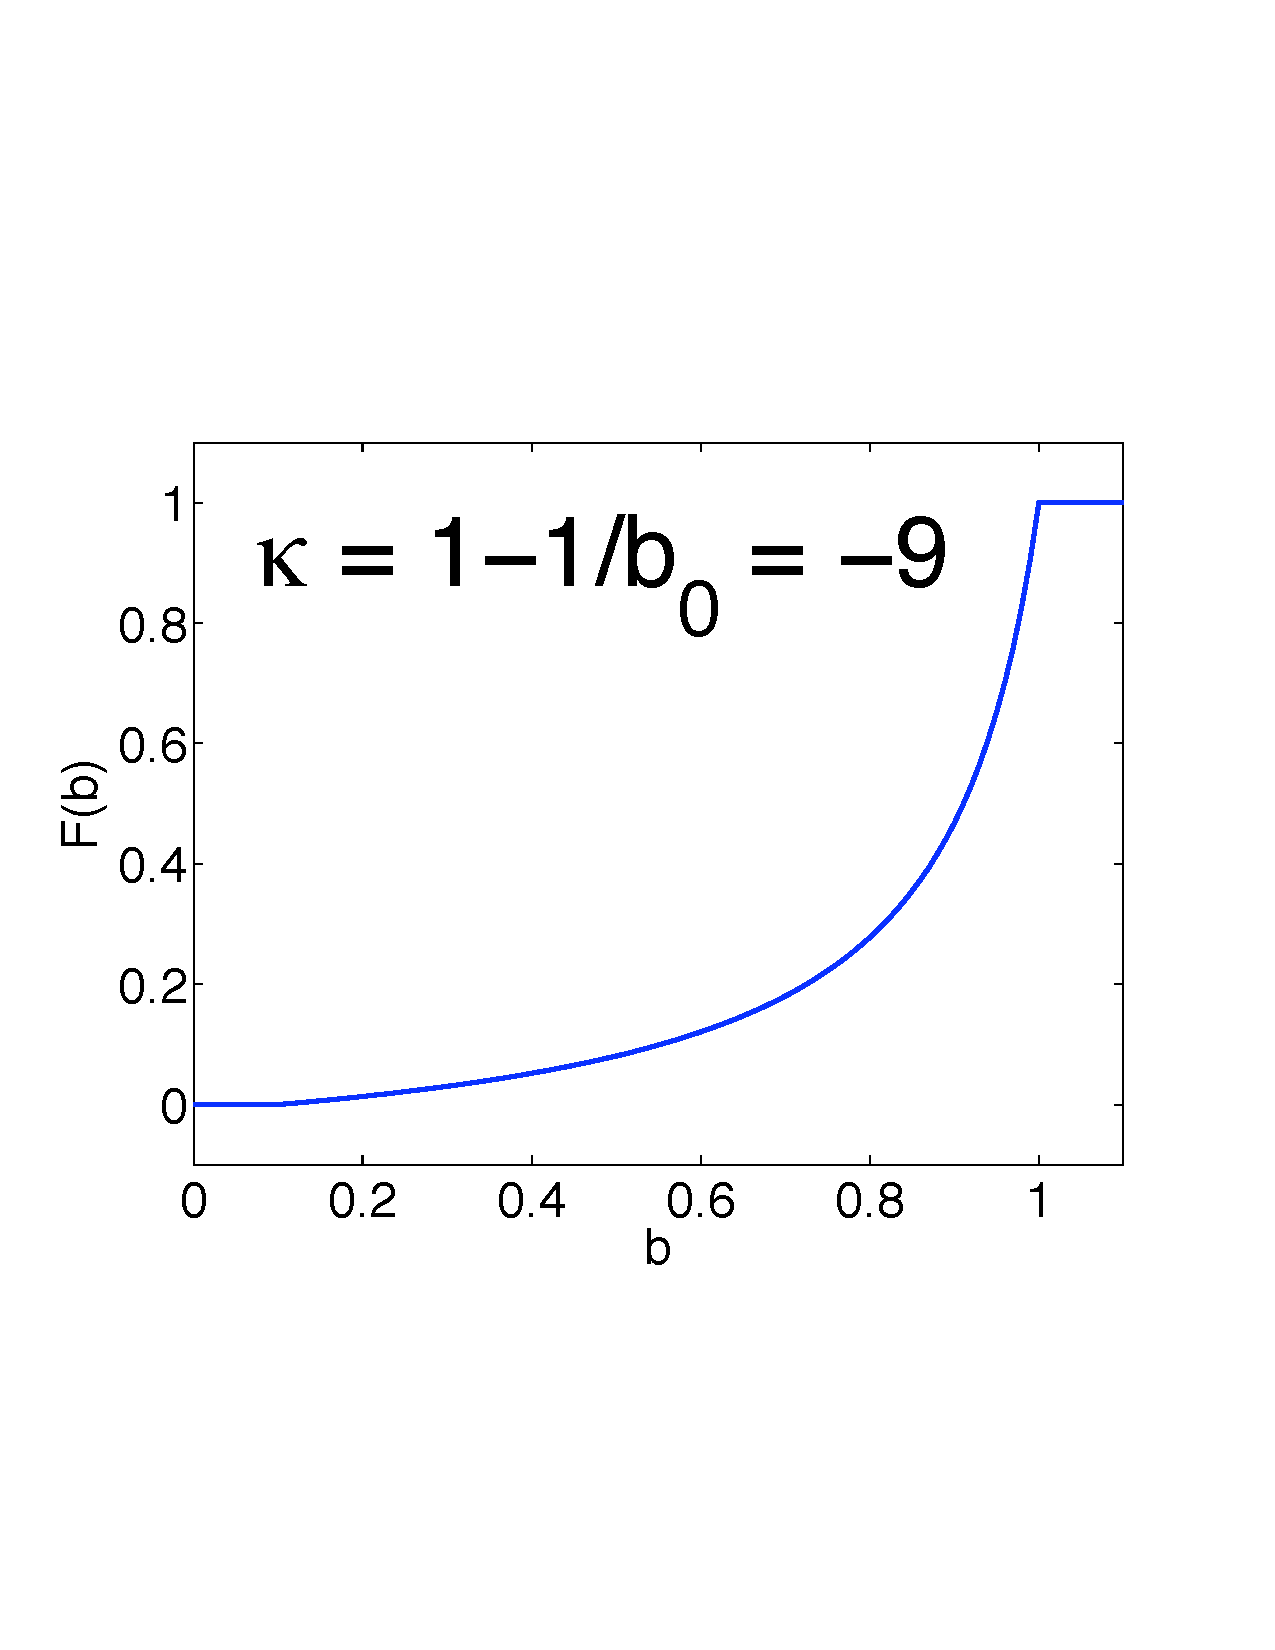
\includegraphics[width=2.25in]{figures/Fconcaveup.pdf} & 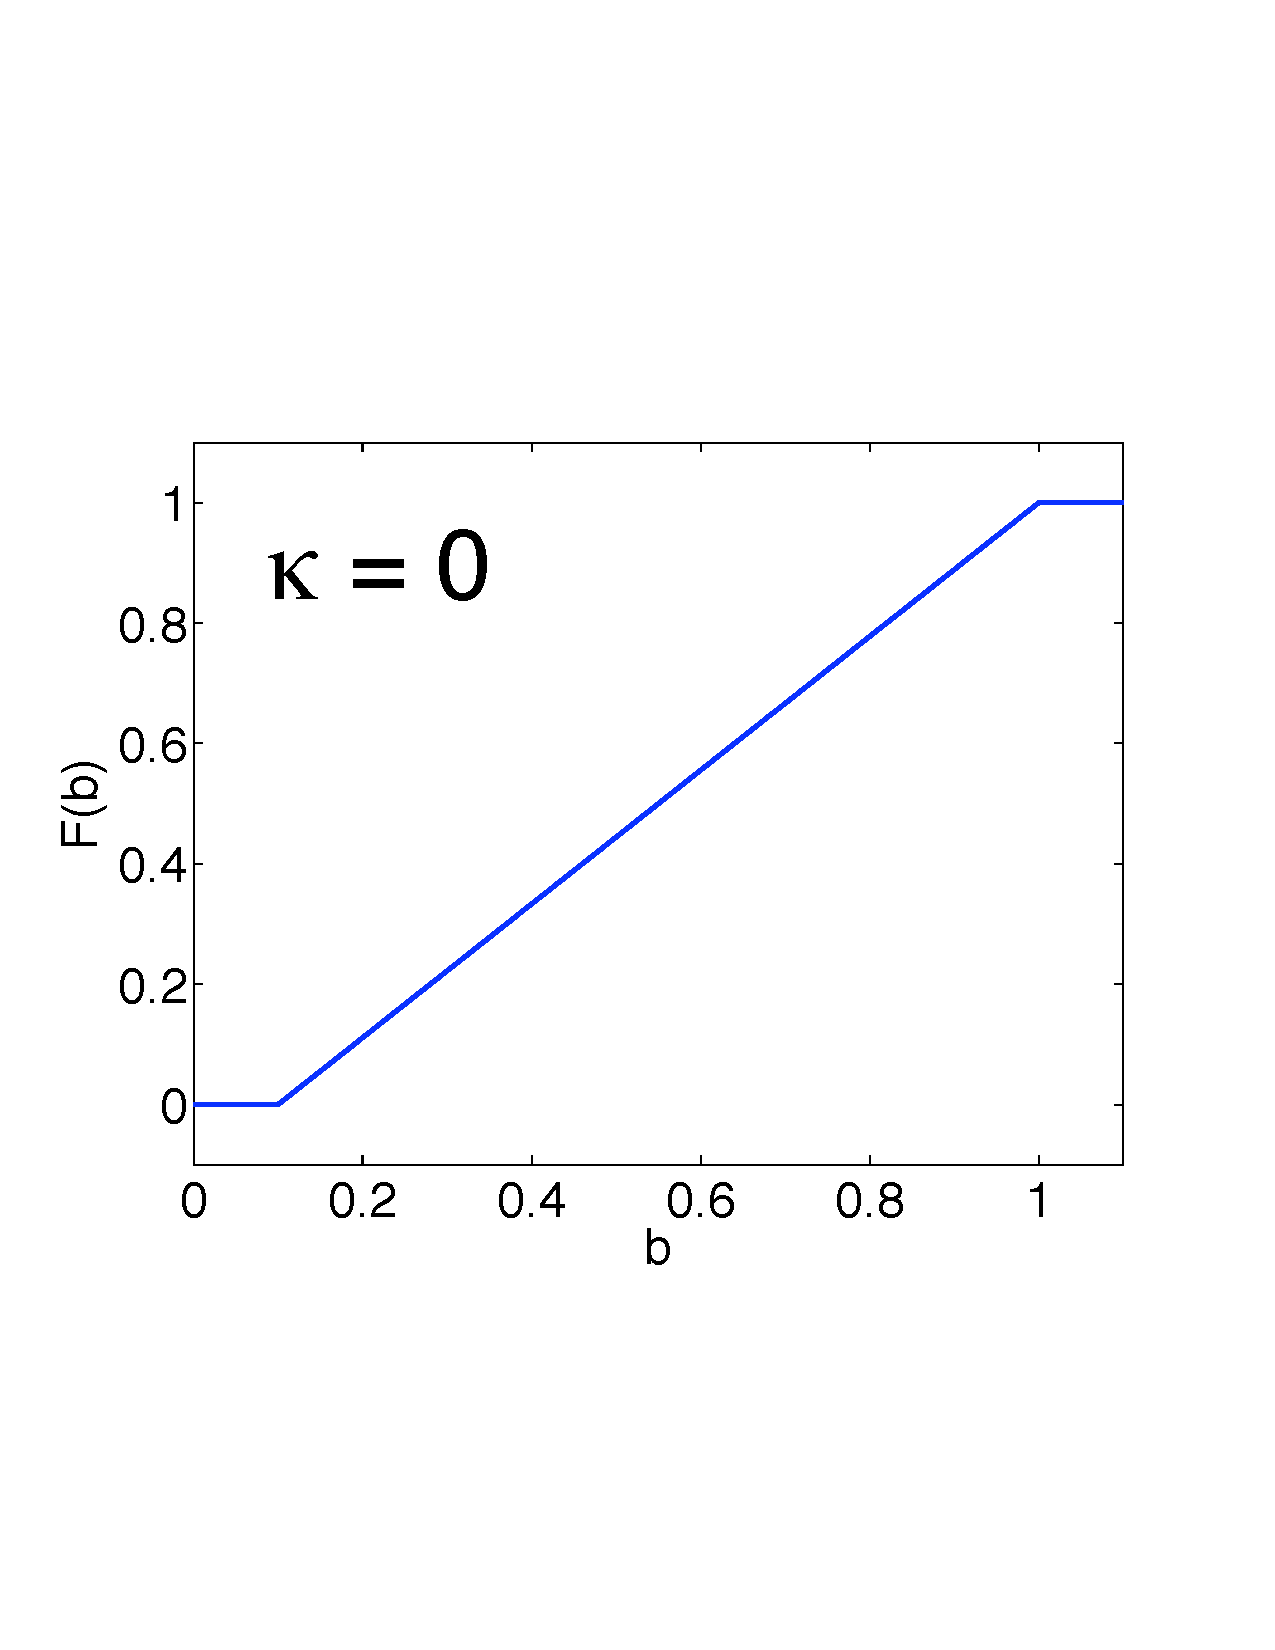
\includegraphics[width=2.25in]{figures/Flinear.pdf} & 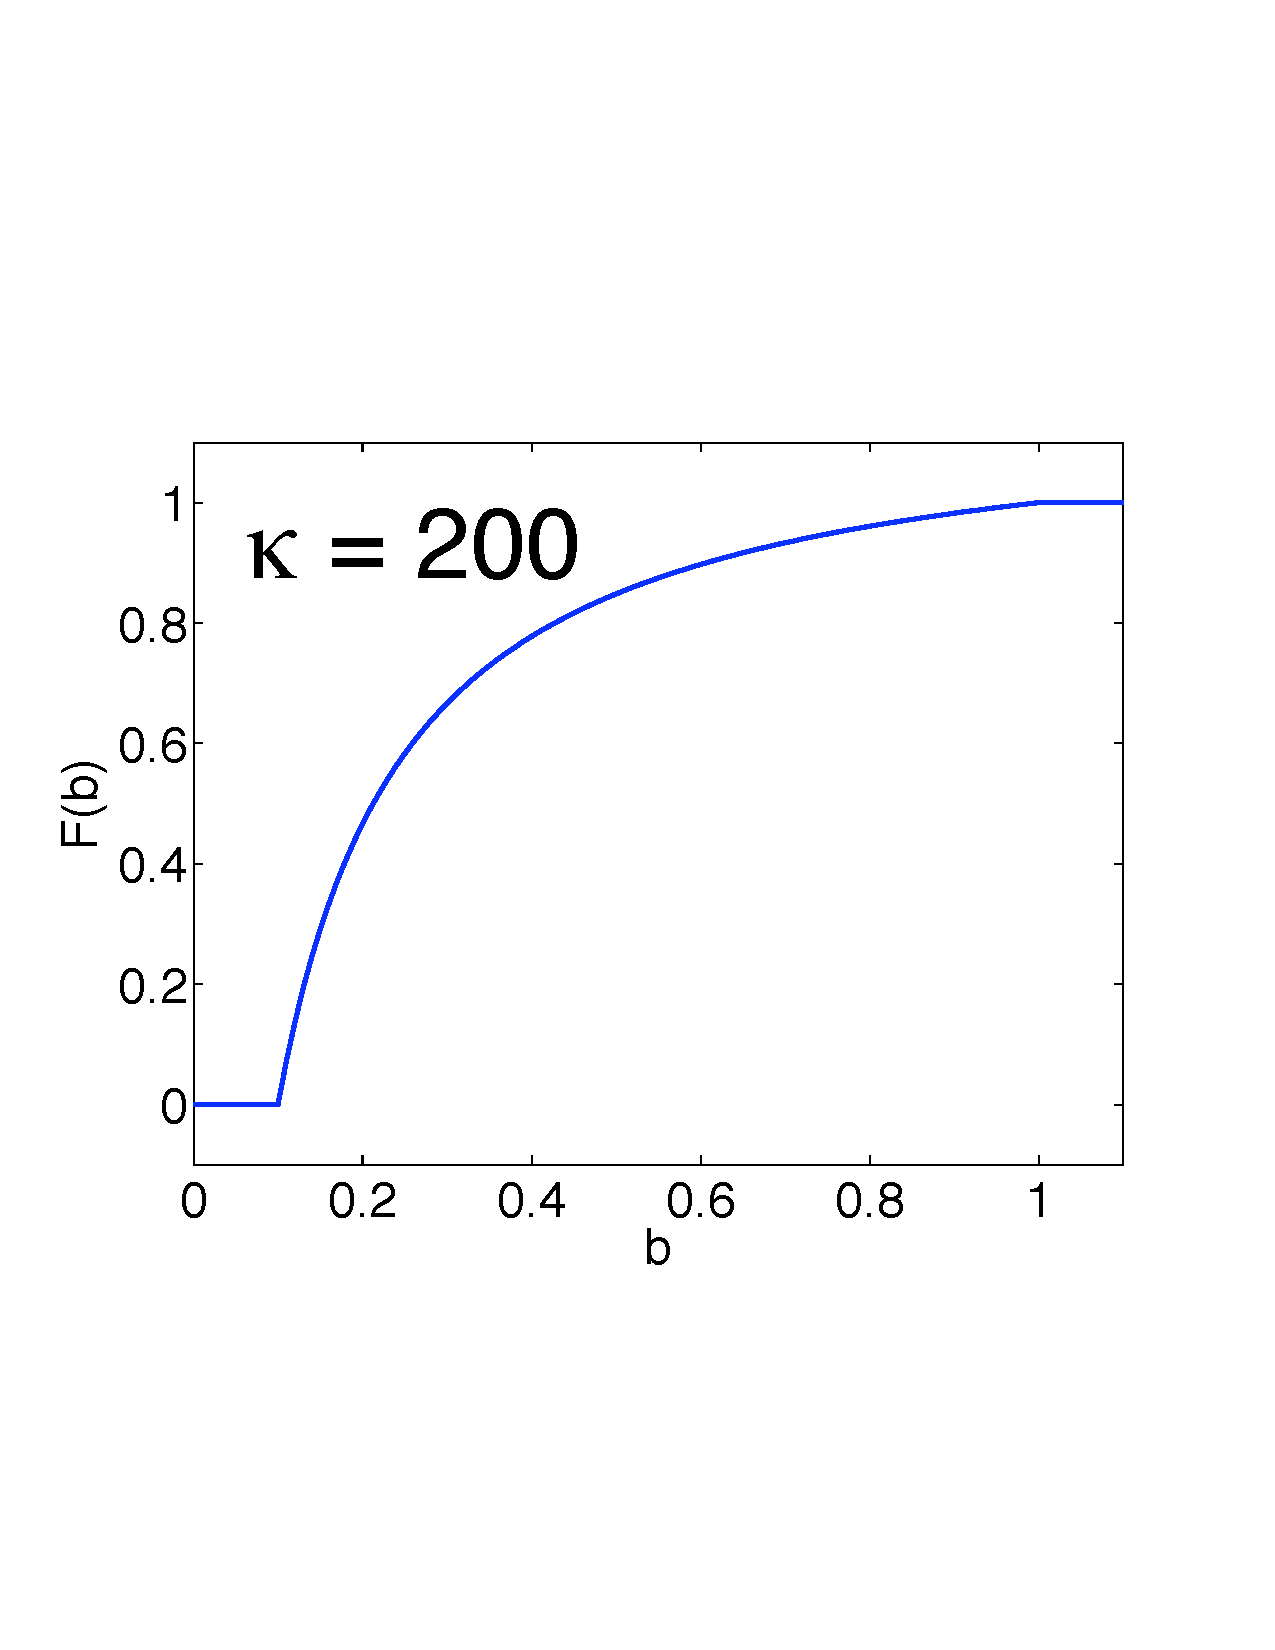
\includegraphics[width=2.25in]{figures/Fconcavedown.pdf}
\end{tabular}
\mycaption{
The shape of transition function \ref{eqn:functional} as a function of the normalized concentration gradient $b$ 
is controlled by the parameter $\kappa$.  When $\kappa < 0 $, $F(b)$ is convex and the mosquito is slow to respond to lower concentration gradients.  When $\kappa >0 $, $F(b)$ is concave and the mosquito is quicker to respond to lower concentration gradients.  
For these figures, $b_0 = 0.1$.
\comment{These three figures would be better if they were combined to create a single larger figure with three curves for $\alpha$ instead of 3 plots for $F$.}
}
\label{fig:exampleF}
\end{figure}

\begin{figure}[hbt]
\centering
 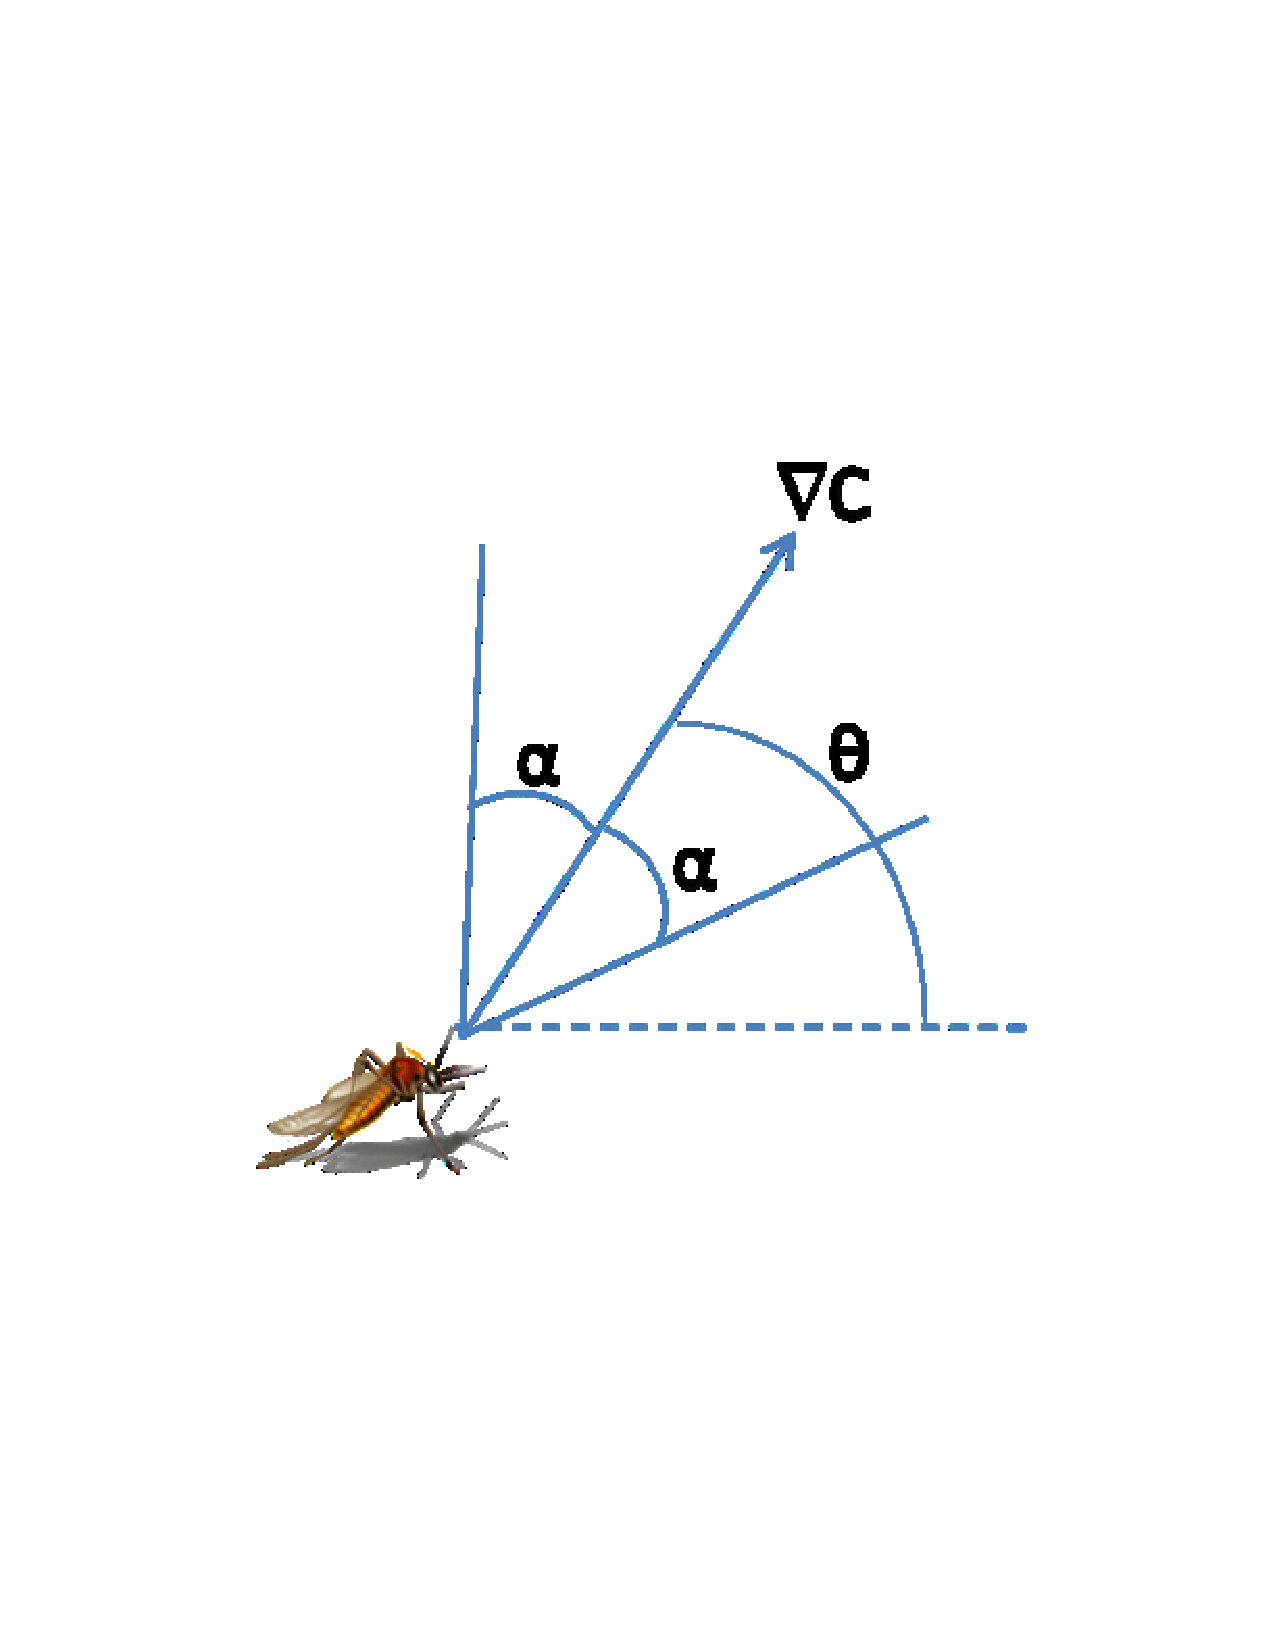
\includegraphics[width=2.0in]{figures/GradientWalkSchematic.pdf}
\mycaption{Schematic of the mosquito host-seeking model based on the concentration gradient direction. At each discrete time step, the angle $\Theta$ for the direction that a mosquito is flying can change by as much as the angle $\alpha$, as defined in equation \ref{eqn:response}. }

\label{MosquitoGradient}
\end{figure}

Let $G_{sat}$ be the maximum concentration gradient that can be sensed and define the 
normalized gradient at  the mosquito location by $b = |\nabla C|/G_{sat}$.  Let the threshold 
concentration gradient be a proportion of the saturation gradient $G_0 = b_0\ G_{sat}$ and 
let $\kappa$ be any number in the range
$(-1/b_0,\infty)$.  The window $[\theta-\alpha,\theta+\alpha]$ (see Fig.~\ref{MosquitoGradient}) is computed from
\begin{equation} \label{eqn:response}
\alpha = \alpha_{max} - (\alpha_{max}-\alpha_{min}) F(b,b_0;\kappa)
\end{equation}
where $\alpha_{max}$ and $\alpha_{min}$ are free parameters and the transition function is set to
\begin{equation}
F(b, b_0; \kappa) = \left\{ \begin{array}{lr} 
   0, & b < b_0 \\ 
   \dfrac{(1+\kappa b_0)(b-b_0)}{(1+\kappa b_0 b)(1 - b_0)}, & b_0 \leq b \leq 1 \\ 
   1, & 1 < b  
   \end{array}\right. . \label{eqn:functional}
 \end{equation}



\subsubsection{Concentration values}  
A different modeling approach to the way a mosquito may take a step based on the CO$_2$ concentration 
is to use only the value of the concentration, not the gradient. This equivalent to a temporal gradient in the 
sense that the current concentration value must be compared to the previous value it encountered in order
to decide on the target direction.  
\begin{itemize}
\item
If the current concentration at the mosquito location is larger than the
concentration at the previous step, the direction used in the previous step becomes the new target direction 
$\theta$.  
\item 
If the current concentration at the mosquito location is lower than the
concentration at the previous step, the target direction is set to the reverse of the one used in the previous step.
\item
A saturation concentration change $\Delta C_{sat}$ is used as the maximum concentration
change that can be sensed.  A threshold concentration change $\Delta C_0 = b_0\ \Delta C_{sat}$ 
is also used so that very small changes in concentration values are imperceptible.  
\end{itemize}
A window of directions centered around $\theta$ is computed as before except that the gradient
magnitude is replaced by the difference $C(x,y,t_n)-C(x,y,t_{n-1})$.  The window of possible step
directions is given by Eq.~(\ref{eqn:response}), where $b = |C(x,y,t_n)-C(x,y,t_{n-1})|/\Delta C_{sat}$.

	

	
	
\subsubsection{Wind velocity} 
%
We model the wind sensing capability of the mosquitoes as a ``precision window'' around the direction of the wind, where the stochasticity of the agent response is intended to mimic the average behavior that would occur based on visual cues over many possible ground patterns.  In our model, the wind velocity is known either as a function or at 
least on grid points.  It is then straightforward to calculate the wind direction at the mosquito locations from interpolated grid values.   As before, we choose a random direction within the precision window. We assume that the mosquitoes fly at speeds greater than the mean wind speed, so that upwind flight is possible. 	

Let $\theta_v$ be the direction of the wind $\vec V$ at the mosquito location.
When $C < C_0$, the mosquito exhibits ranging flight behavior and its target direction, $\theta = \theta_v + \psi$, depends on their assigned flight strategy: $\psi=0$ for downwind flight, $\psi=\pi$ for upwind flight, and $\psi \in [-\pi/2, -\pi/4] \cup [\pi/4,\pi/2]$ for varying degrees of crosswind flight.  As before, the direction is chosen randomly from a window
$[\theta-\alpha,\theta+\alpha]$ where $\alpha$ is given by Eq.~(\ref{eqn:response}) with $b = |\vec{V}|/V_{sat}$ and the threshold speed by $V_0 = b_0\ V_{sat}$: 
\begin{equation*}
	\theta_w \in [\theta_v + \psi-\alpha,\theta_v + \psi+\alpha]. %\label{eqn:vdirchoice}
\end{equation*}

During crosswind ranging behavior, a mosquito will oscillate between traveling to the right and left of the wind direction. The duration of the travel in one direction is a free parameter in the model. We choose this duration to be uniformly selected from an interval $T_{cwd} = [T_{min},T_{max}]$. 


\subsubsection{Flying velocity} 
%
We assume that the speed of a mosquito is bounded between a minimum $S_{min}$ and a 
maximum $S_{max}$.  Unlike the stochasticity in the choice of direction, the speed of the 
step taken by a mosquito is found through the deterministic formula
\begin{equation}\label{eqn:speed}
	s = S_{max} - (S_{max} -  S_{min})F(b, b_0; \kappa).
\end{equation}
where the variable $b$ represents the normalized CO$_2$ concentration $C/C_{sat}$ at the mosquito location.  Because of the
nature of the function $F(b, b_0; \kappa)$, depicted in Figure~\ref{fig:exampleF}, if the concentration 
is below the threshold $C_0$, the mosquito speed becomes $S_{max}$.  The mosquito
speed may be set to a constant by simply choosing $S_{min} = S_{max}$.


\subsubsection{Summary of mosquito behavior model}
%
Each time a mosquito takes a step, the model determines the direction of the step and the speed of the mosquito.
The direction of the step is given by a random variable chosen from a uniform distribution in
the interval $[\theta-\alpha,\theta+\alpha]$. The speed varies with the CO$_2$ concentration. 

In ranging flight, when there are no concentration cues, the 
target direction $\theta = \theta_v + \psi$ is determined by the wind velocity direction and ranging behavior.  The size $\alpha$ of the interval is
computed with Eq.~(\ref{eqn:response}) with $b = |\vec{V}|/V_{sat}$. The updated mosquito position is given by
\begin{eqnarray}
	\begin{pmatrix} x_{n+1} \\ y_{n+1} \end{pmatrix} &=& 
	\begin{pmatrix} x_n \\ y_n \end{pmatrix} + S_{max}\Delta T \begin{pmatrix}  \cos{\theta_w} \\ \sin{\theta_w} \end{pmatrix} + \vec{V}\Delta T , \label{eq:wind:motion}
\end{eqnarray}
where $\Delta T$ is the time between mosquito decisions, as distinct from the time step for the advection-diffusion equation, $\Delta t$. The last term is passive advection of the mosquito in the ambient wind.

In homing flight, when the concentration is above threshold, the motion from upwind flight ($\psi = \pi$) and up-gradient flight is averaged together.
The speed of the step is computed deterministically using Eq.~(\ref{eqn:speed}). The updated mosquito position is given by
\begin{eqnarray}
	\begin{pmatrix} x_{n+1} \\ y_{n+1} \end{pmatrix} &=& 
	\begin{pmatrix} x_n \\ y_n \end{pmatrix} + \frac{s(x_n,y_n)\Delta T}{2} \begin{pmatrix}  \cos{\theta_w} + \cos{\theta_c}\\ \sin{\theta_w} + \sin{\theta_c} \end{pmatrix}  + \vec{V}\Delta T . \label{eq:both:motion}
\end{eqnarray}

%%%%%%%%%%%%%%%	
\subsection{Dimensionless formulation}
%%%%%%%%%%%%%%%%
We nondimensionalize the problem using a typical mosquito speed of $s_0 = 1$ m/s~\cite{Clements1999} and a time interval of 
$\tau = 0.1$ s in which mosquitoes make navigation decisions. This latter number is the fastest time scale in Figure 5 from Dekker et al. (2005) (see specifically panel B on the right), although longer time scales look plausible as well.  These scales together imply a typical mosquito flight length of $L = s_0 \tau = 0.1$ m, which we use to scale all length variables.  
In addition, we scale the concentration using the characteristic value $C_{sat}$, the saturation level for mosquito sensing, which we take to be 1250 ppm (1.25e-3 units CO$_2$ per unit air) for this work.
In dimensionless form, Eq.~(\ref{eq:conv-diff}) becomes
\begin{equation}\label{eq:conv-diff2}
\frac{\partial \hat{C}}{\partial \hat{t}} + \nabla\cdot ( \vec{\hat{V}} \hat{C} ) = \nu\nabla^2 \hat{C} + \hat{C}_s(x,y),
\end{equation}
where $\nu = D/\tau s_0^2$ and the source term is $\hat{C}_s(x,y) = \hat{J}_0 \int\!\!\!\int \delta(x-x_h-z_1,y-y_h-z_2) dz_1 dz_2$ with $\hat{J}_0 =\tau J_0/C_{sat}$.
Equations~\eqref{eq:wind:motion} and \eqref{eq:both:motion} are nondimensionalized in a straightforward fashion by $s_0$, $L$, and $\tau$. 
All numerical simulations are computed using dimensionless variables.







 
\section{Chemotaxis Rules in Homing Flight}\label{sec:chemostats}
%%%%%%%%%%%%%%%%
	
		
Our framework can model chemotaxis of mosquitos seeking their host by either sensing the absolute amount of CO$_2$ or its gradients to adjust its direction and speed.  A natural question to ask is if these choices
lead to significantly different results or if they are similar in some sense.  In this example we investigate this 
question statistically to conclude that in some measure different choices lead to results without statistically
significant differences. That is, we found that there were different chemotaxis rule sets, based on either the local concentration of CO$_2$ or its gradients,  that gave similar results.  

	In each example we followed the same procedure: 
\begin{enumerate}
	\item
	\textbf{Specification of a test problem:} We consider a simplified problem with a steady CO$_2$ concentration and no wind. 
	We define a concentration given by $C(x,y) = e^{-10(x^2+y^2)}$ that does not change in time.
	Two hundred mosquitoes are randomly distributed initially in the rectangle $0.15\times 0.05$ centered over the $x$-axis 
	and located 0.55 units above the origin. In this rectangle, the CO$_2$ concentration ranges from 2.5-4.9\% of the maximum. The mosquitoes do 
	not interact with each other and they do not affect the chemical distribution. We assume a mosquito has found the host when it comes within a critical radius of $r_c = $ 0.2 units of
	the source. Mosquitoes that have done this are assigned a distance of zero (during post-processing) for the rest of the 
	simulation.
\item
\textbf{Simulations:} For each simulation using a particular rule set A, we release 200 mosquitoes and compute the 
distance from each one to the center of the concentration plume at every step.  This leads to a time-dependent
distribution of distances, which can be displayed as a histogram at each moment in time. To estimate the variability one can 
expect from running different instances of the same rule set A, we repeat the simulation 25 distinct times.
\item
\textbf{Statistical analysis:} For each simulation, we use the mosquito distances to compute a normalized cumulative distribution function (CDF) for each moment in time
(see Fig.~\ref{fig:diffhist}). We then compute the maximum distance between CDFs for each pair of
simulations at each time step. This is the two-sided Kolmogorov-Smirnov (KS) statistic. For $n=25$ simulations, this gives us $n(n-1)/2 = 300$ KS statistics within a rule set at each time.
We then find the mean of the KS statistics and compute an empirical 95\% confidence interval.  \textit{This interval provides a sense of the variability of rule set A
and a baseline for comparing other rule sets to it.} 
\item
\textbf{Conclusions:} We now calculate KS statistics between rule set A and a new rule set B, for a total of $n^2$ values at each moment in time. \textit{If the mean of these statistics falls outside the 95\% confidence interval of the variability of rule set A, we conclude that the two rules show statistically significant differences.} 
\end{enumerate}

\subsubsection{Diffusion of Mosquitoes}
We first consider unbiased diffusion of mosquitoes as an example. Diffusion is governed by a random direction 
at each time step and a fixed speed of $S_{min} = S_{max} = 1$. Figure~\ref{fig:diffhist} shows the 
distance histograms and corresponding cumulative distribution functions for one diffusion simulation (200 mosquitoes) at 
selected times. From the CDFs we may construct an empirical distribution for diffusion KS statistics
as described in step 3 above (black curve and vertical bars in the left panel of Fig.~\ref{fig:diffcomp}).


\begin{figure}[htp]
	\begin{center}
		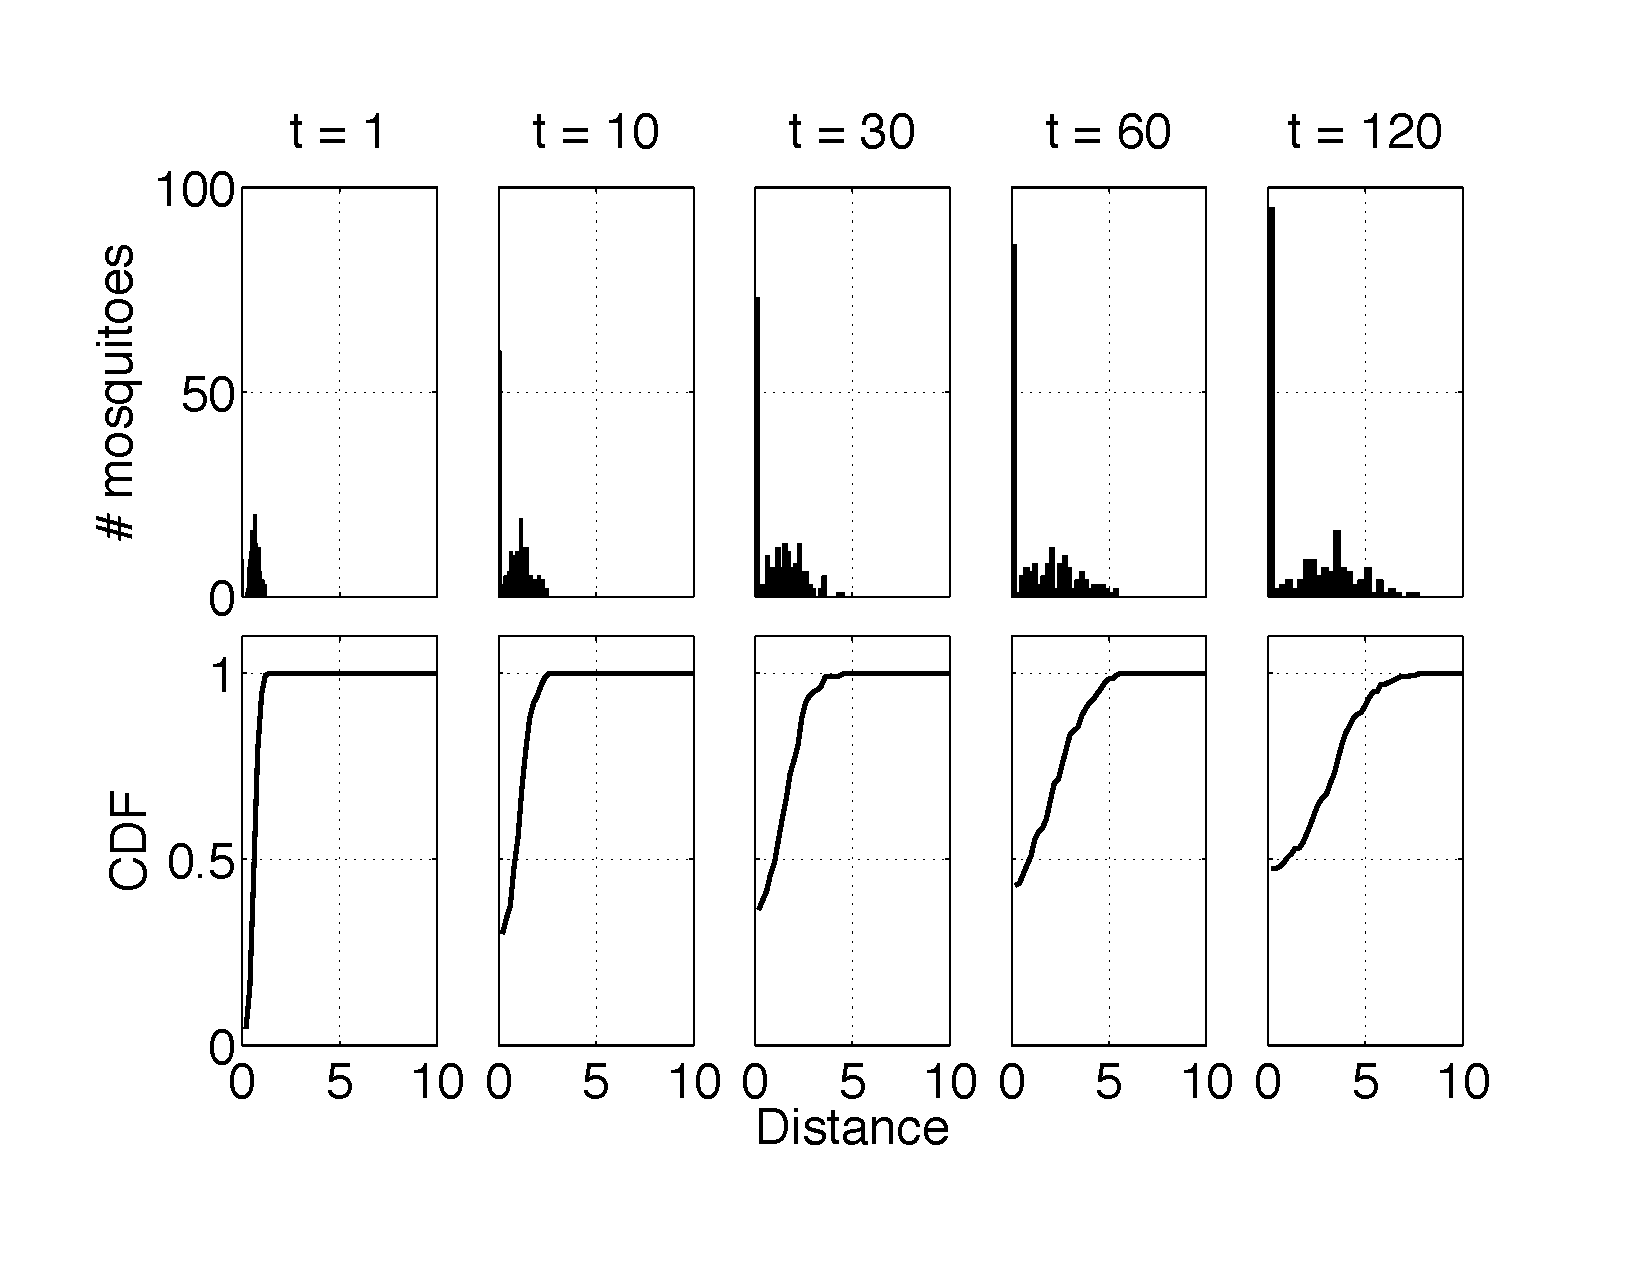
\includegraphics[width=6.8in]{figures/DiffusionFigure.pdf}
	\end{center}
	\mycaption{The distribution (upper panels) and normalized cumulative distribution (lower panels) of mosquito distances (meters) to the CO$_2$ source over time (seconds) assuming passive diffusion. Nearly half of the mosquitoes have found the source after 120 s, while the mean of the remaining mosquito distances increases with time. The CDFs will be used to calculate KS statistics within and between different rule sets.}\label{fig:diffhist}
\end{figure}

\begin{table}[hbt]
	\mycaption{Parameters for the chemotaxis homing flight rules. The $R_g$ rule set us based on knowledge of the gradient of the concentration in all directions. The $R_c$ rule set us based on the rate of change of CO$_2$ concentration sensed by the mosquito along its flight path (directional derivative).  }
	\begin{center}
		\begin{tabular}{cc}
			{\begin{tabular}{|c|c|c|c|}
				\hline
				\multicolumn{4}{|c|}{$R_g$}\\
				\hline
				\multicolumn{2}{|c|}{Direction} & \multicolumn{2}{|c|}{Speed} \\
				\multicolumn{2}{|c|}{$b=|\nabla C|/G_{sat}$} & \multicolumn{2}{|c|}{$b=C/C_{sat}$} \\
				\hline
				$\alpha_{min}$ & $\pi/2$ &    $S_{min}$ & 0.1 \\
				$\alpha_{max}$ & $\pi$ &      $S_{max}$ & 1.9 \\
				$G_0$ & 0.0833 &              $C_0$ & 0.05 \\
				$G_{sat}$ & 1.7 &             $C_{sat}$ & 0.9 \\
			    $\kappa$ & 0 &            	$\kappa$ & 0 \\
				\hline
			\end{tabular}} &
			{\begin{tabular}{|c|c|c|c|}
				\hline
				\multicolumn{4}{|c|}{$R_c$}\\
				\hline
				\multicolumn{2}{|c|}{Direction} & \multicolumn{2}{|c|}{Speed} \\
				\multicolumn{2}{|c|}{$b=\Delta C/\Delta C_{sat}$} & \multicolumn{2}{|c|}{$b=C/C_{sat}$} \\
				\hline
				$\alpha_{min}$ & $\pi/12$ &    $S_{min}$ & 0.1 \\
				$\alpha_{max}$ & $\pi$ &      $S_{max}$ & 1.9 \\
				$\Delta C_0$ & 0.0042 &              $C_0$ & 0.05 \\
				$\Delta C_{sat}$ & 0.17 &             $C_{sat}$ & 0.9 \\
			    $\kappa$ & 0 &            	$\kappa$ & 0 \\
				\hline
			\end{tabular}} 		
	\end{tabular}\label{tab:toyparams1}
	\end{center}
\end{table}
		
We compare diffusion with rule $R_g$ in Table~\ref{tab:toyparams1}. Under $R_g$, mosquitoes use the CO$_2$ gradient to choose direction and the concentration to choose speed. Note from the table that far from the CO$_2$ 
source, where concentration is below the threshold, mosquitoes move faster under rule $R_g$ 
(at $S_{max}$) than the diffusion speed of 1.
We calculated the mean KS statistic over time between diffusion and $R_g$ (left panel in Fig.~\ref{fig:diffcomp}, red line) and see that these two heuristics are significantly different as expected. Under $R_g$, many more mosquitoes find the source. 
		
\begin{figure}[hbtp]
	\begin{center}
		\begin{tabular}{cc}
		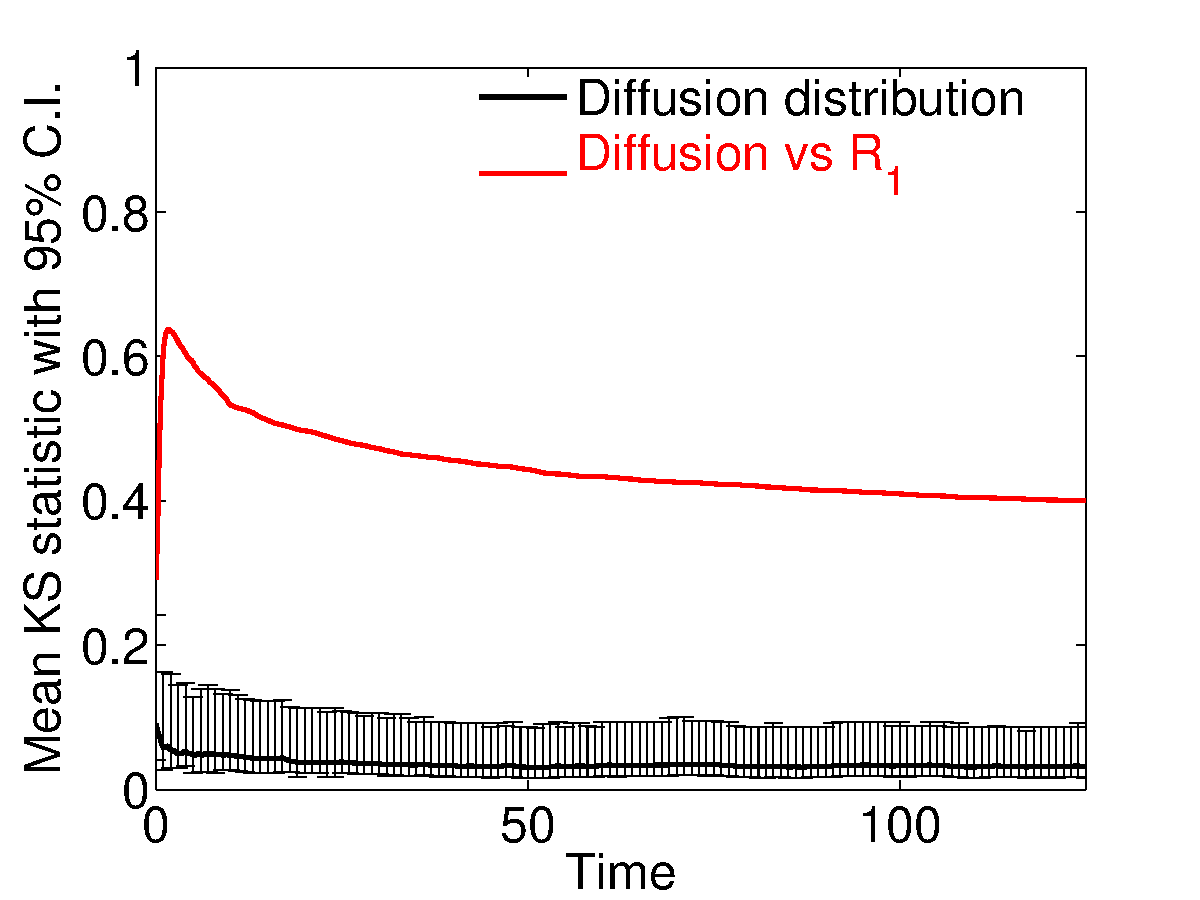
\includegraphics[width=3.25in]{figures/DiffusionComparison.pdf} & 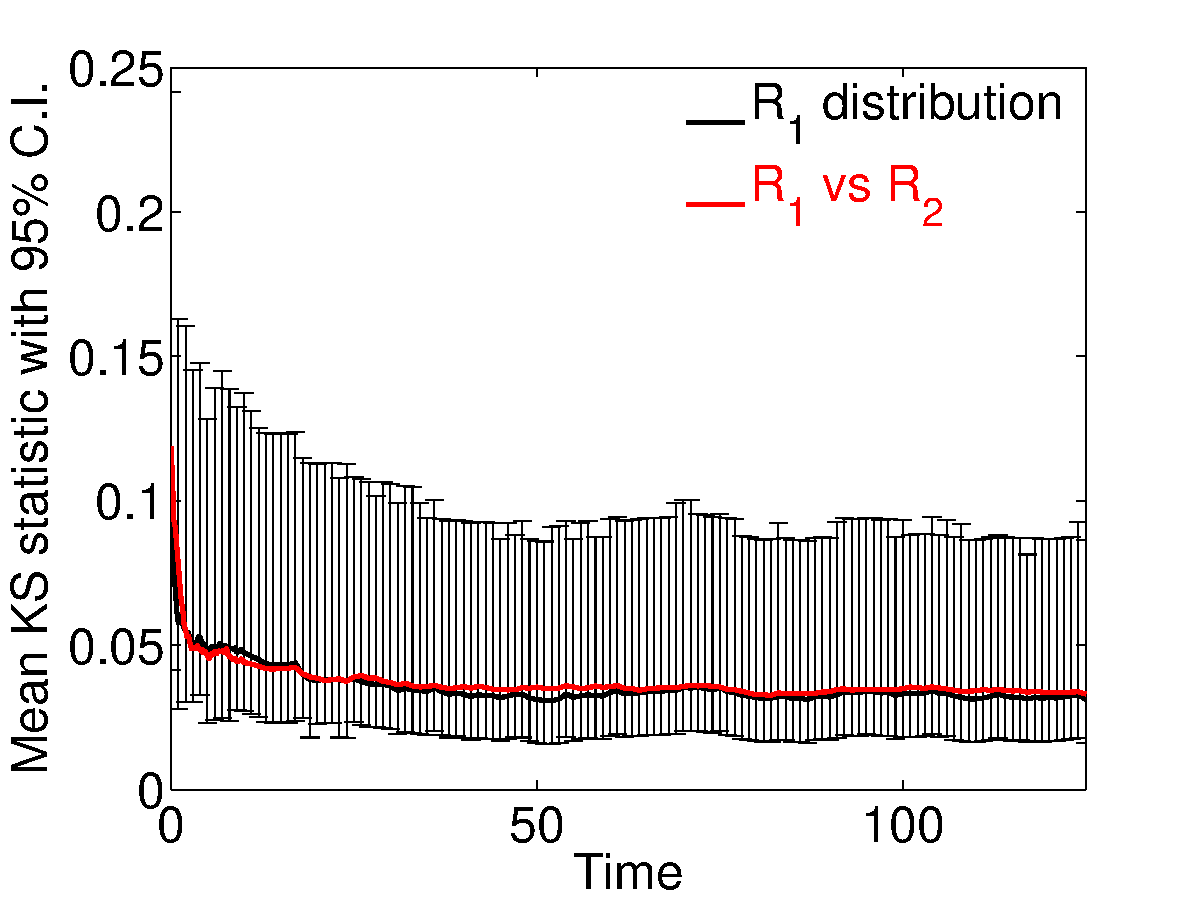
\includegraphics[width=3.25in]{figures/R1Comp.pdf}
	\end{tabular}
	\end{center}
	\mycaption{Left panel: Diffusion vs $R_g$ with parameters from Table~\ref{tab:toyparams1}. The black lines are the mean and 95\% confidence interval of all the pairwise KS statistics calculated within the diffusion simulations. The red line is the mean of the KS statistics calculated between diffusion and $R_g$. Since the red line falls so far from the diffusion confidence interval, we conclude that the two rules are highly dissimilar. Right panel: $R_g$ vs $R_c$ from Table~\ref{tab:toyparams1}. Now the black lines are the empirical distribution for $R_g$, and the red line is the mean of the KS statistics between $R_g$ and $R_c$. Unlike the left panel, these two rules are nearly identical.}\label{fig:diffcomp}
\end{figure}

\subsubsection{Comparison of Chemotaxis Rules}

We also compare different chemotaxis rules to each other. Figure~\ref{fig:diffcomp} (right panel) shows a comparison between rules $R_g$ and $R_c$ (see Table~\ref{tab:toyparams1}), which exhibit nearly identical behavior using the mean KS statistic. Mosquitoes using $R_c$ do not sense the CO$_2$ gradient. Instead, they compare the current concentration to the concentration at their previous location, which gives them an estimate of the gradient in their
current heading direction only (a directional derivative). In contrast, mosquitoes using $R_g$ know the gradient direction and are much more efficient in reaching the CO$_2$ source. However, if we choose the minimum window width $\alpha_{min}$ to be much lower for $R_c$ than $R_g$, then the rules are indistinguishable. The threshold and saturation levels for the rules are related by $\Delta C_0 = G_0L/2$ and $\Delta C_{sat} = G_{sat}L$. 


The observations we made while studying the model include:
\begin{itemize}
\item
Consider rule set $R_g$ in Table~\ref{tab:toyparams1} and compare it to a new rule set $R_{gf}$  that uses 
the same variable $b = |\nabla C|/G_{sat}$ to choose the step direction but uses a fixed step speed
$S_{max} = S_{min} = 1$.  We can find parameter values for $\alpha_{min}$, $S_{min}$ and $S_{max}$
in $R_g$ such that the mean KS statistic between $R_g$ and $R_{gf}$ is not significantly different from $R_g$.  A similar conclusion is reached 
based on $R_c$ instead of $R_g$.

	\item
	We could not find parameter values that matched $R_c$ to $R_{gf}$ (or $R_g$ to $R_{cf}$ in the analogous case). We conclude that rules differing in both direction and speed may be difficult or impossible to match, although this may not hold under a broader parameter search.
	\item
	If the free parameters $\alpha_{min}$, $S_{min}$, and $S_{max}$ are varied between rules without keeping the same proportionality, then the mean KS statistic sensitively changes (we fix $\alpha_{max}$ at $\pi$ to ensure diffusive behavior far from the source). The same is true for independent variation of the thresholds and saturation levels. The match between $R_g$ and $R_c$ shows mixed sensitivity and robustness to other parameter changes: 
	\begin{itemize}
		\item
		Doubling the time step makes no substantial difference to the resulting match. Halving the time step causes a noticeable but not significant mismatch at early times.
		\item
		Doubling the critical radius $r_c$ where the mosquitoes find the source does not affect the match, but halving it causes a significant mismatch at early times. 
		\item
		Upward concavity ($\kappa = 1 - 1/b_0$) makes no substantial difference to the resulting match. Downward concavity of the response function ($\kappa = 200$) causes a significant mismatch at early times. 
	\end{itemize}
\end{itemize}



\textbf{Final parameter choices:} We choose to have our mosquito agents use the spatial gradient to determine direction.  Figure~\ref{fig:diffcomp} (right panel) shows that it is possible, through appropriate parameter choices, to make a rule based on the spatial gradient indistinguishable from one that uses more limited information. We may capture a wide range of potential behaviors by varying parameters, although other chemotaxis models may be easily substituted for this one. The specific chemotaxis parameters that we use for the full wind driven simulations are listed in Table~\ref{tab:finalparams}. We always choose the concavity parameter $\kappa$ to be 0, corresponding to a piecewise linear response.


%%%%%%%%%%%%%%%	
\section{Sensitivity Analysis}

Our goal is to explore the effect of host spatial distribution on the mosquito-host contact rate. To do this, we must fix a large number of parameter values governing the odor plume simulation and the mosquito behavior (see Table~\ref{tab:finalparams}). In this section, we consider a single host distribution and locally vary a collection of our model parameters independently to assess the robustness of the model with respect to our target parameter set. 

We vary each of the starred parameters in Table~\ref{tab:finalparams} by $\pm$10\% while holding all other parameters constant. Figure~\ref{fig:2groups} shows the fixed arrangement of hosts for the local sensitivity analysis. Ten birds are divided into two groups, seven on the left and three on the right, with approximately the same density in each group. We also choose a single sequence of random velocity fields in time to superpose over the bulk flow. In order to capture the average mosquito behavior, the simulations are repeated $n$ times within each ranging behavior (upwind, downwind, and crosswind), until a mild convergence criterion is satisfied ($n \approx$ 15-20). The same sequence of random numbers are used generate mosquito behavior in each set of $n$ simulations. The differences in mosquito behavior between sets will be due solely to the parameter perturbations and not to the stochastic nature of the agents.


\begin{figure}[hbt]
	\centering
 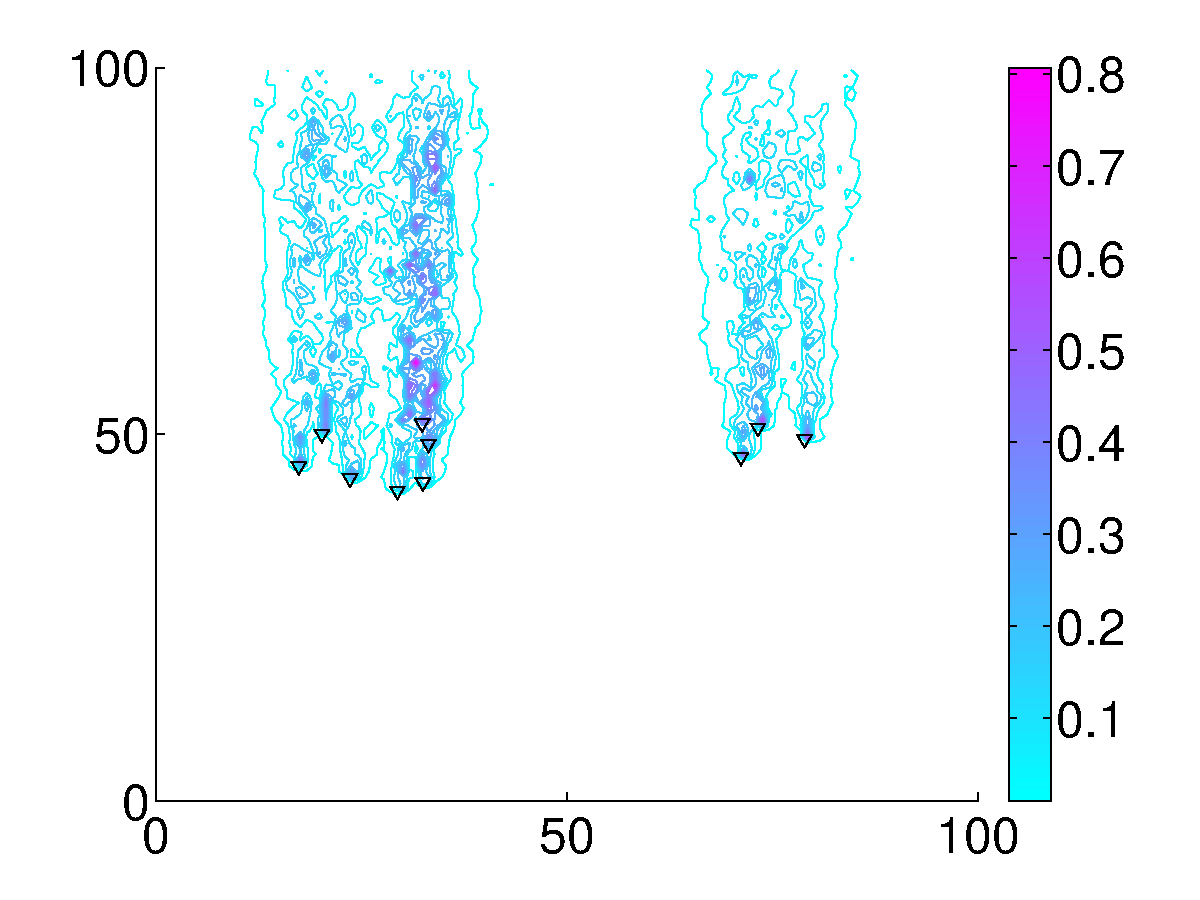
\includegraphics[width=5.0in]{figures/2groups.pdf} 

\mycaption{Fixed distribution of hosts for the local sensitivity analysis: seven hosts on the left and three on the right. The colorbar denotes nondimensional concentration. Here $L_x = L_y=100$, $N_x= N_y=128$, $\Delta t = 0.01$ for the advection-diffusion equation, and $\Delta T = 1$ for the mosquito motion. 
}
\label{fig:2groups}
\end{figure}
		


The output variables we analyzed include: 
\begin{itemize}
\item the proportion of mosquitoes that find a host anywhere in the domain, $P_{tot}$, 
\item the proportion that find the left group, $P_\ell$, and 
\item the proportion that find the right group, $P_r = P_{tot} - P_\ell$. 
\end{itemize}

If we denote a generic input variable by $I$, its unperturbed value as $I^0$, and its perturbations as $I^\pm$, then our sensitivity index ($SI$) is calculated as 
\begin{equation*}
	SI = \frac{P_*^+ - P_*^-}{I^+ - I^-}I^0 = \frac{P_*^+ - P_*^-}{0.2},
\end{equation*}
which is a centered difference approximation of the derivative of the output with respect to the normalized input. We estimate the error in this method by 
\begin{equation*}
	E = \left|\frac{P_*^+ - P_*^0}{0.1} - \frac{P_*^0 - P_*^-}{0.1} \right|,
\end{equation*}
which is the difference of the one-sided derivatives. 

We show our most sensitive results in Table~\ref{tab:sensitivity}. Consider the first row, which is looking at the sensitivity of $P_{tot}$ with respect to $S_{max}$ when the mosquitoes have crosswind ranging flight behavior. The baseline value for $P_{tot}$ is about 80\%. The sensitivity index is 0.1517, which means that if $S_{max}$ is varied by 10\%, then approximately 1.5\% more mosquitoes will locate a host, plus or minus 0.6\% (0.1*Error/2). Our highest sensitivities show changes of 1-2\% of the total mosquito population with a 10\% input change. A 1-2\% change on a scale of 35-80\% indicates that our model is locally robust to our parameter set of choice. We do not characterize the variability with respect to stochastic effects.

\begin{table}[hbtp]
	\mycaption{Nondimensional parameter choices. *Starred values were locally varied.}
	\begin{center}
		\begin{tabular}{|c|c|c|}
			\hline
			\multicolumn{3}{|c|}{Mosquito speed in the presence of CO$_2$, $b=C/C_{sat}$} \\
			\hline
			$S_{min}$ & 0.4* & minimum mosquito flight speed\\
			$S_{max}$ & 1.5* & maximum mosquito flight speed\\
			$C_0$ & 0.01* & CO$_2$ sensing threshold\\
			$C_{sat}$ & 1 & CO$_2$ sensing saturation \\
			\hline
			\multicolumn{3}{|c|}{Mosquito CO$_2$ direction, $b=|\nabla C|/G_{sat}$} \\
			\hline
			$\alpha_{min}$ & $\pi/6$* & minimum interval width for sensing $\nabla C$\\
			$\alpha_{max}$ & $\pi$  & maximum interval width for sensing $\nabla C$\\
			$G_0$ & $C_0/10$  & gradient sensing threshold\\
			$G_{sat}$ & $(C_{sat}-C_0)/5$  & gradient sensing saturation\\
			\hline
			\multicolumn{3}{|c|}{Mosquito wind direction, $b=|\vec{V}|/V_{sat}$} \\
			 \hline
			$\alpha_{min}$ & $\pi/6$* & minimum interval width for sensing wind direction \\
			$\alpha_{max}$ & $\pi/2$ & maximum interval width for sensing wind direction \\
			$V_0$ & 0 & wind sensing threshold\\
			$V_{sat}$ & 0.5 & wind sensing saturation\\
			\hline
			\multicolumn{3}{|c|}{Wind parameters} \\
			\hline
			$\vec{U}$ & [0,0.2] & bulk flow\\
			$\vec{U}_r$ & [X(t),Y(t)]0.15* & superposed random flow field \\
			\multirow{2}{*}{$X(t),Y(t)$} & \multirow{2}{*}{mean 0, std dev 0.5} & normally distributed random variables \\  
			& & changed every 20 $\Delta T$ \\
			\hline
			\multicolumn{3}{|c|}{Miscellaneous constants} \\
			\hline
			$\nu$ & 1.6e-4* & diffusion coefficient\\
			$\hat{J_0}$ & 0.1333* & source coefficient\\
			$r_c$ & 5* & critical radius for mosquito removal from simulation \\
			\multirow{2}{*}{$T_{cwd}$} & \multirow{2}{*}{$\Delta T$[5,9]*} & duration of crosswind flight in one direction\\
			& & uniformly selected from the interval \\
			$N_v$ & 200 & number of mosquitoes per simulation \\
			$N_h$ & 10 & number of hosts per simulation \\
			\hline
		\end{tabular}
	\end{center}\label{tab:finalparams}
\end{table}

\begin{table}[hbtp]
	\mycaption{Most sensitive local variation.}
	\begin{center}
		\begin{tabular}{|c|c|c|c|c|}
			\hline
			Ranging behavior & input & output (baseline value)& $SI$ & Error \\
			\hline
			\multirow{5}{*}{crosswind} & \multirow{2}{*}{$S_{max}$} & $P_{tot}$ (80.2\%) & 0.1517 & 0.1064 \\
										& 						  & $P_\ell$ (44.5\%)	& 0.1050 & 0.0579 \\  
										\cline{2-5}   
										 & \multirow{3}{*}{$T_{cwd}$} & $P_{tot}$ (80.2\%) & 0.2178 & 0.0502 \\
										& 						  & $P_\ell$	(44.5\%) & 0.1016 & 0.0280 \\
										& 						  & $P_r$ (35.6\%)	& 0.1163 & 0.0222 \\
			\hline
			\multirow{2}{*}{downwind} & $S_{max}$ & $P_{tot}$ (57.6\%) & 0.1250 & 0.0536 \\
										 & $r_c$ & $P_{tot}$ (57.6\%) & 0.1230 & 0.0045  \\
			\hline
		\end{tabular}
	\end{center}\label{tab:sensitivity}
\end{table}



\section{Model Simulations}
 \comment{\it  {\bf  Each simulation is carefully chosen to answer a specific question.  Begin the example by stating the question you are addressing, follow with the simulation/experiment and end with how this example  gives insight into answering the question.  
 Every figure should also make a specific point, which is clearly stated in the figure caption. Check that you include enough details so the experiments could be reproduced, but do not include unnecessary details and include only brief outlines of methods well described elsewhere. 
}}


	\notes{\it  {\bf Here is a suggested format for each example. }}
	
	\notes{\it  {\bf The question  we are addressing is ... }}
		
	\notes{\it  {\bf The simulation we used to investigate this question is to ... }}
	
	\notes{\it  {\bf In these simulations we found that ... }}
	
        \notes{\it  {\bf This means that ... }}
	

\subsection{Host-seeking Flight Behavior and Wind Direction}
	How the effectiveness of the different host-seeking strategies depends on the wind velocity. 
Simulations varying mosquito ranging flight behavior (crosswind, downwind, upwind)

\subsection{Distribution of Hosts }
Simulations varying the number of hosts in each group or the volume in which there are a fixed number of hosts (can do this with one and two groups)

\subsection{Host Density and Host-seeking Flight Behavior }
Plots of resultant per capita biting rate with respect to ranging flight behavior and host density (and host location within a group?)




\section{Summary and Discussion}
	 \comment{\it  {\bf Summarize your key findings in the first paragraph of the Discussion. Start by answering the question posed in introduction and relating your results to existing knowledge.}}
	 	 
We developed a new hybrid agent-based/continuum model to explore the effect of spatial 
heterogeneity on the encounter rate between mosquito vectors and bird hosts.  
The flight direction and speed of individual mosquitoes is influenced by both the wind and odors emitted by the hosts.    The odor plumes emitted by the hosts were tracked by an advection-diffusion equation 
with stochastic variations in a directional wind. 
We formulated and compared different strategies that mosquitoes might use to chemotactically locate hosts by using the odor plume  in different 
wind conditions.   

 \comment{\it  {\bf Explicitly discuss (not recapitulate) the results and say what they mean. You may want to highlight, e.g. bullet, the primary results you want the reader to take away from the paper.   
At the end of the summary you may wish to discuss future directions, applications, or generalizations. Restating your key conclusions in different ways helps to reinforce your message.
Provide the reader with your perspective and implications of what the results mean.}}

Our hybrid model is a flexible effective approach to simulate mosquito host-seeking behavior. 


 \comment{\it  {\bf  Put your new results in the context of the overall status of the field.  Explain what is new without exaggerating, and be sure to not just repeat your results. It is fine to reference previous tables and figures. Do not speculate or over discuss results and be sure to discuss weaknesses and discrepancies.  }}
 


 \comment{\it  {\bf  Discuss future extensions of the research.  }}
 
	\begin{itemize}
		\item Discuss applicability of results to parameter choice in current models of vector-borne diseases.
		\item Future directions, two possibilities:
		\begin{itemize}
			\item Couple to a longer time scale model that incorporates transmission, host movement, infection, and death for explicit small scale modeling of disease spread.
			\item Model more complex scenarios (gusting wind, moving hosts, breathing rate) in order to further enhance parameter choice for broader scale SIR models.
		\end{itemize}
	\end{itemize}

I want to tell you that ... list what we learned from our simulations 

\section*{Acknowledgement}
    
 \comment{\it  {\bf Acknowledge and intellectual assistance, technical help, special equipment or materials, and financial assistance (including grants, contracts, or fellowships). 
 }}
This work was supported by ..... 


\bibliographystyle{plain}	
%\newpage  \bibliography{biblio}
\input{biblio.bbl}

% \appendix 
% 
% \section{Robustness to perturbations}\label{app:perturb}
% 
% Here we perform a minor perturbation to the chemical gradient to see how robust our matches from Fig.~\ref{fig:goodmatches} are. We add a small bump to the concentration gradient centered at (0.3, 0.75) that is one-tenth the height of the original, which is still located at (0.4, 0.3). The new chemical concentration is pictured in Fig.~\ref{mosqvizperturb} along with the positions of 200 mosquitoes at various times. Agent paths to the source are shifted toward the perturbation as opposed to the unperturbed case in Fig.~\ref{mosqviz}.
% 
% \begin{figure}[htp]
% \begin{tabular}{cc}
% 	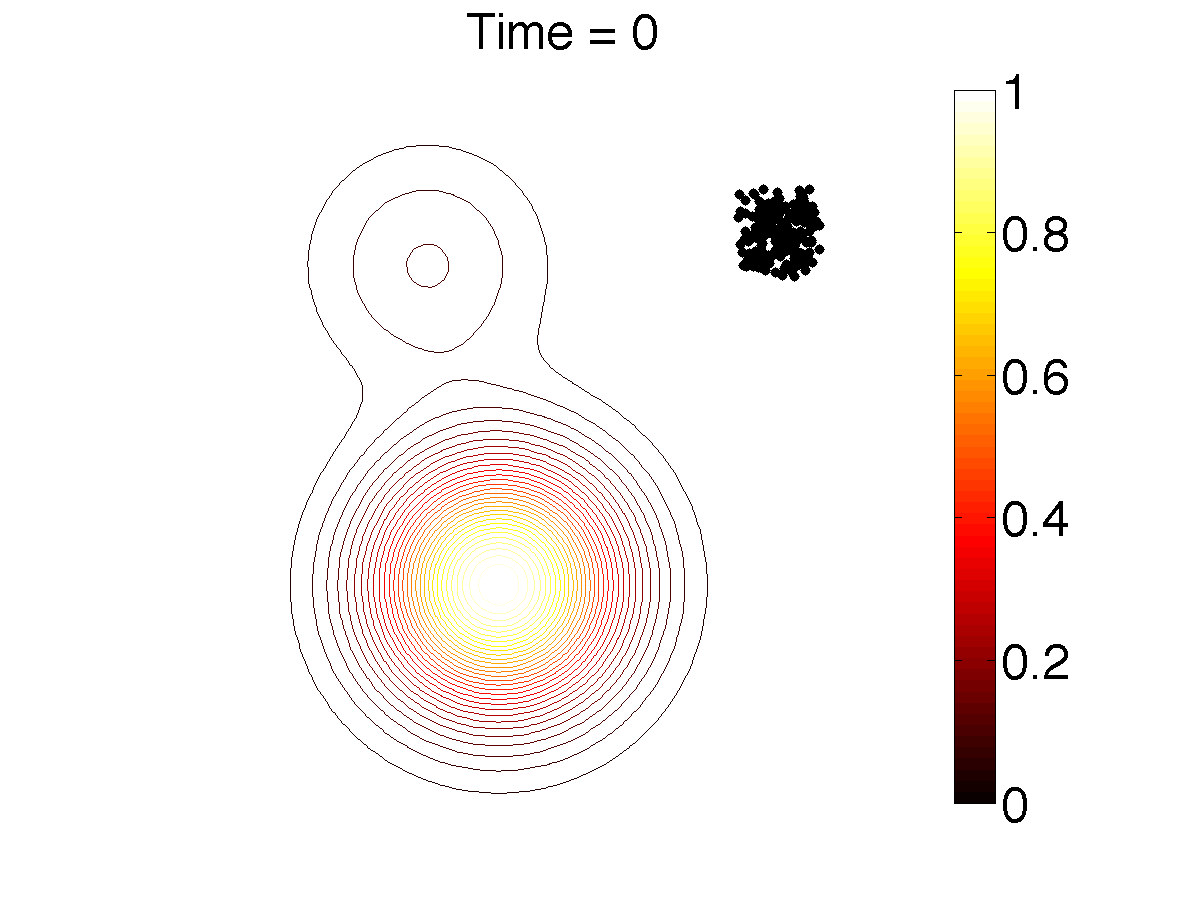
\includegraphics[width=3.25in]{figures/MosqVizPerturb_ruleset01_paramset013_run01_001.png} & 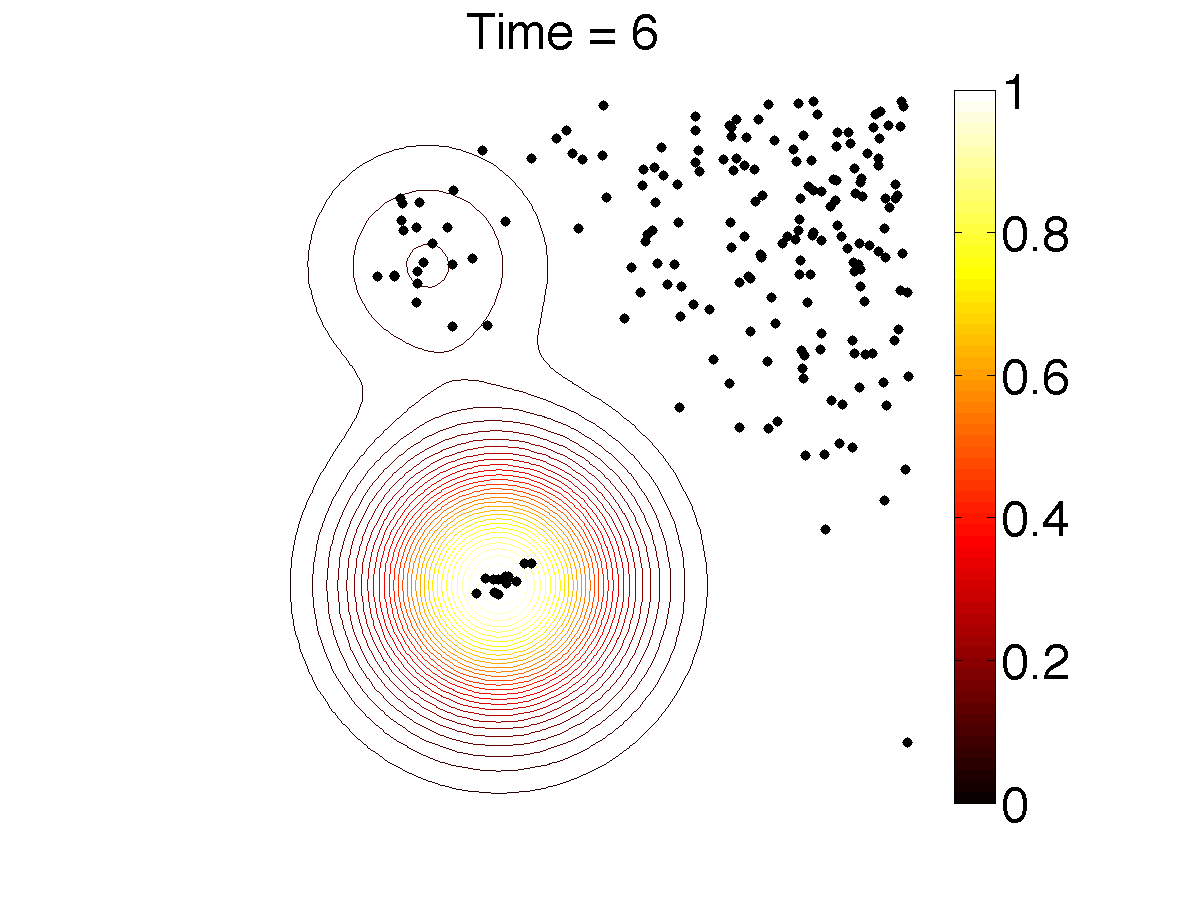
\includegraphics[width=3.25in]{figures/MosqVizPerturb_ruleset01_paramset013_run01_025.png}\\
% 	A & B \\
% 	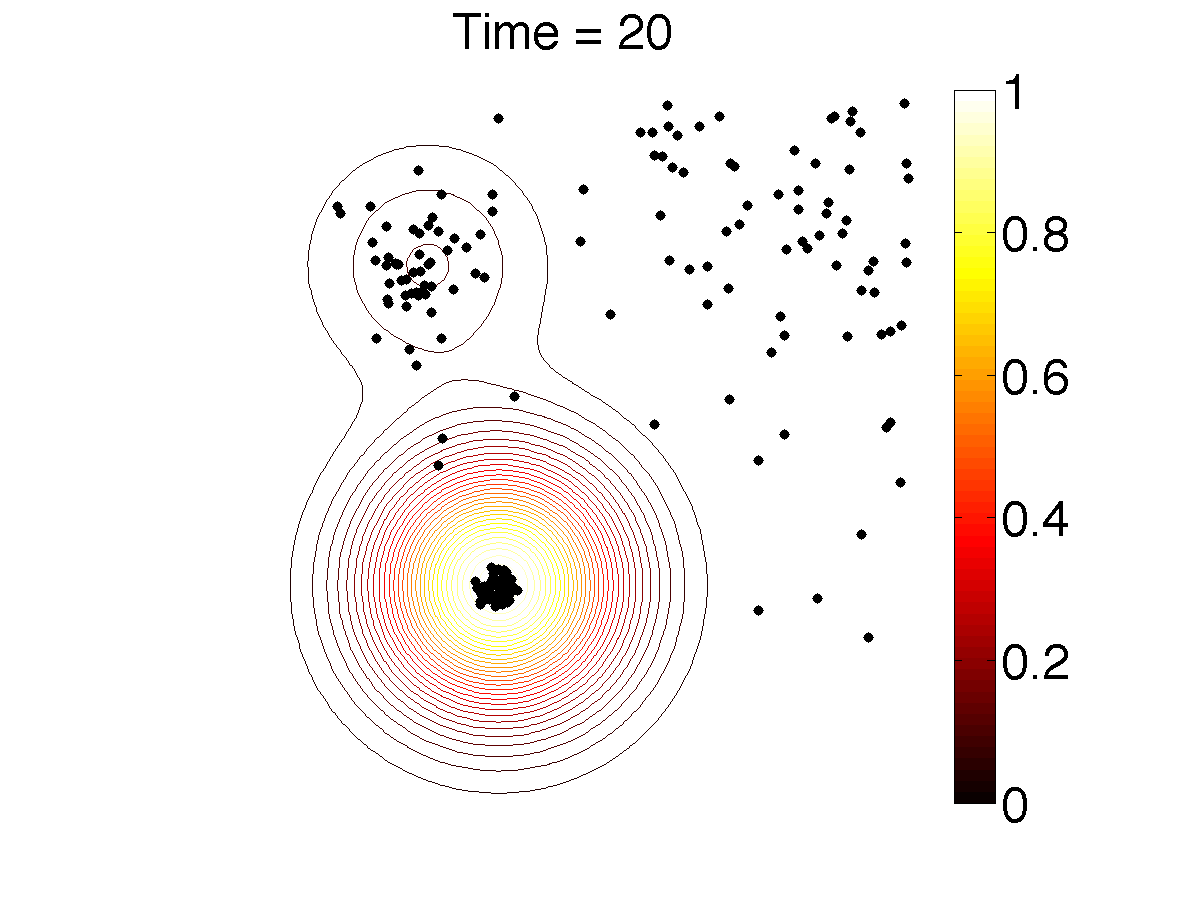
\includegraphics[width=3.25in]{figures/MosqVizPerturb_ruleset01_paramset013_run01_061.png} & 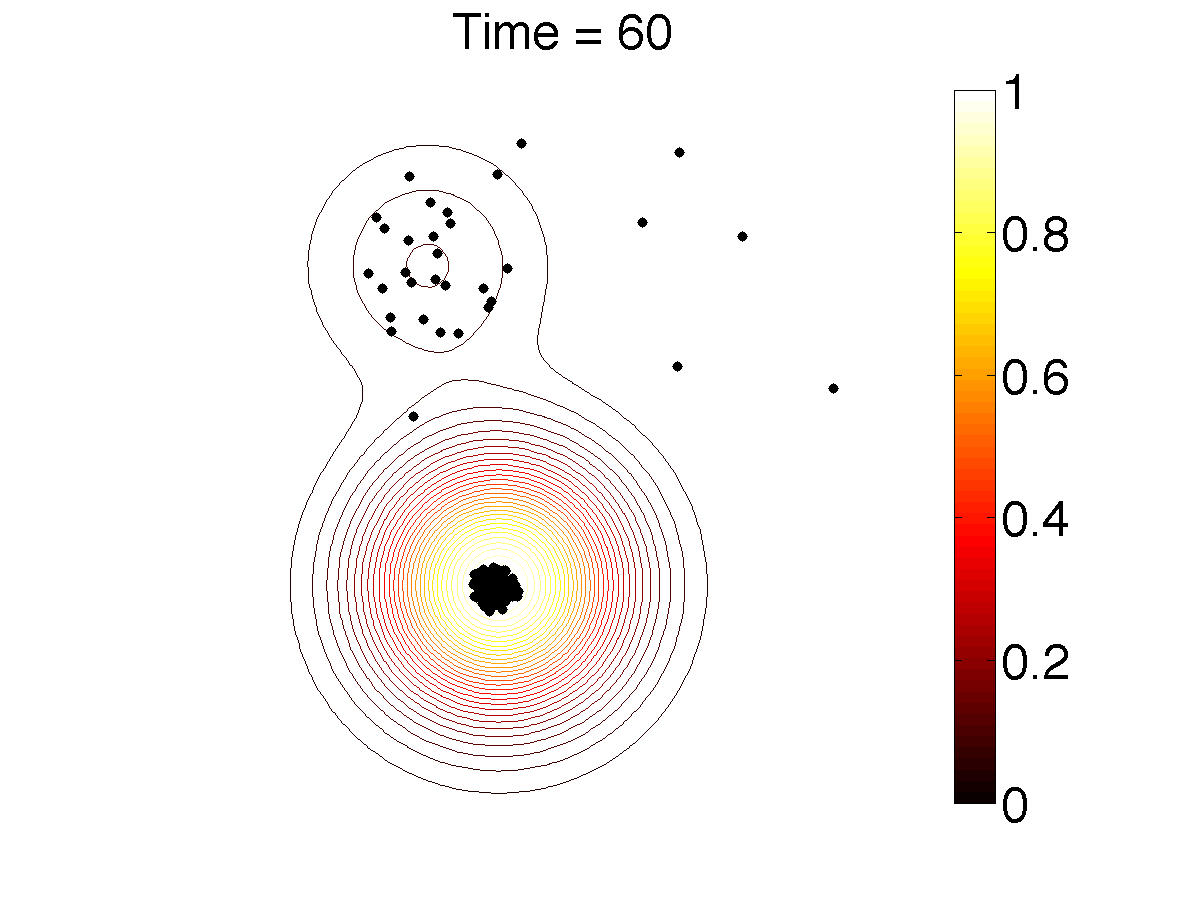
\includegraphics[width=3.25in]{figures/MosqVizPerturb_ruleset01_paramset013_run01_111.png}\\
% 	C & D 
% \end{tabular}
% \caption{Snapshots at various times showing the locations of each of 200 mosquitoes navigating using rule 1 with $\beta_1 = \pi/12$, $S_1 = 0.5$, and $S_2 = 1.25$. The contour plot shows the double-bump chemical concentration. The mosquito agents are clearly influenced by the presence of the second concentration bump.}
% \label{mosqvizperturb}
% \end{figure}
% 
% 
% The best matches to rule 2 were rules 1 and 6 with the parameter sets indicated in the caption in Fig.~\ref{fig:goodmatches}. We re-examine these matches under the perturbed chemical concentration in Fig.~\ref{mosqvizperturb}. The mean KS statistics are shown in Fig.~\ref{ksperturb}, and it can be seen the match with rule 6 is still very good, and the match with rule 1 is still reasonable, although poorer. We conclude that matching rules are reasonably robust to small perturbations.
% 
% \begin{figure}[htp]
% \begin{tabular}{cc}
% 	\multicolumn{2}{c}{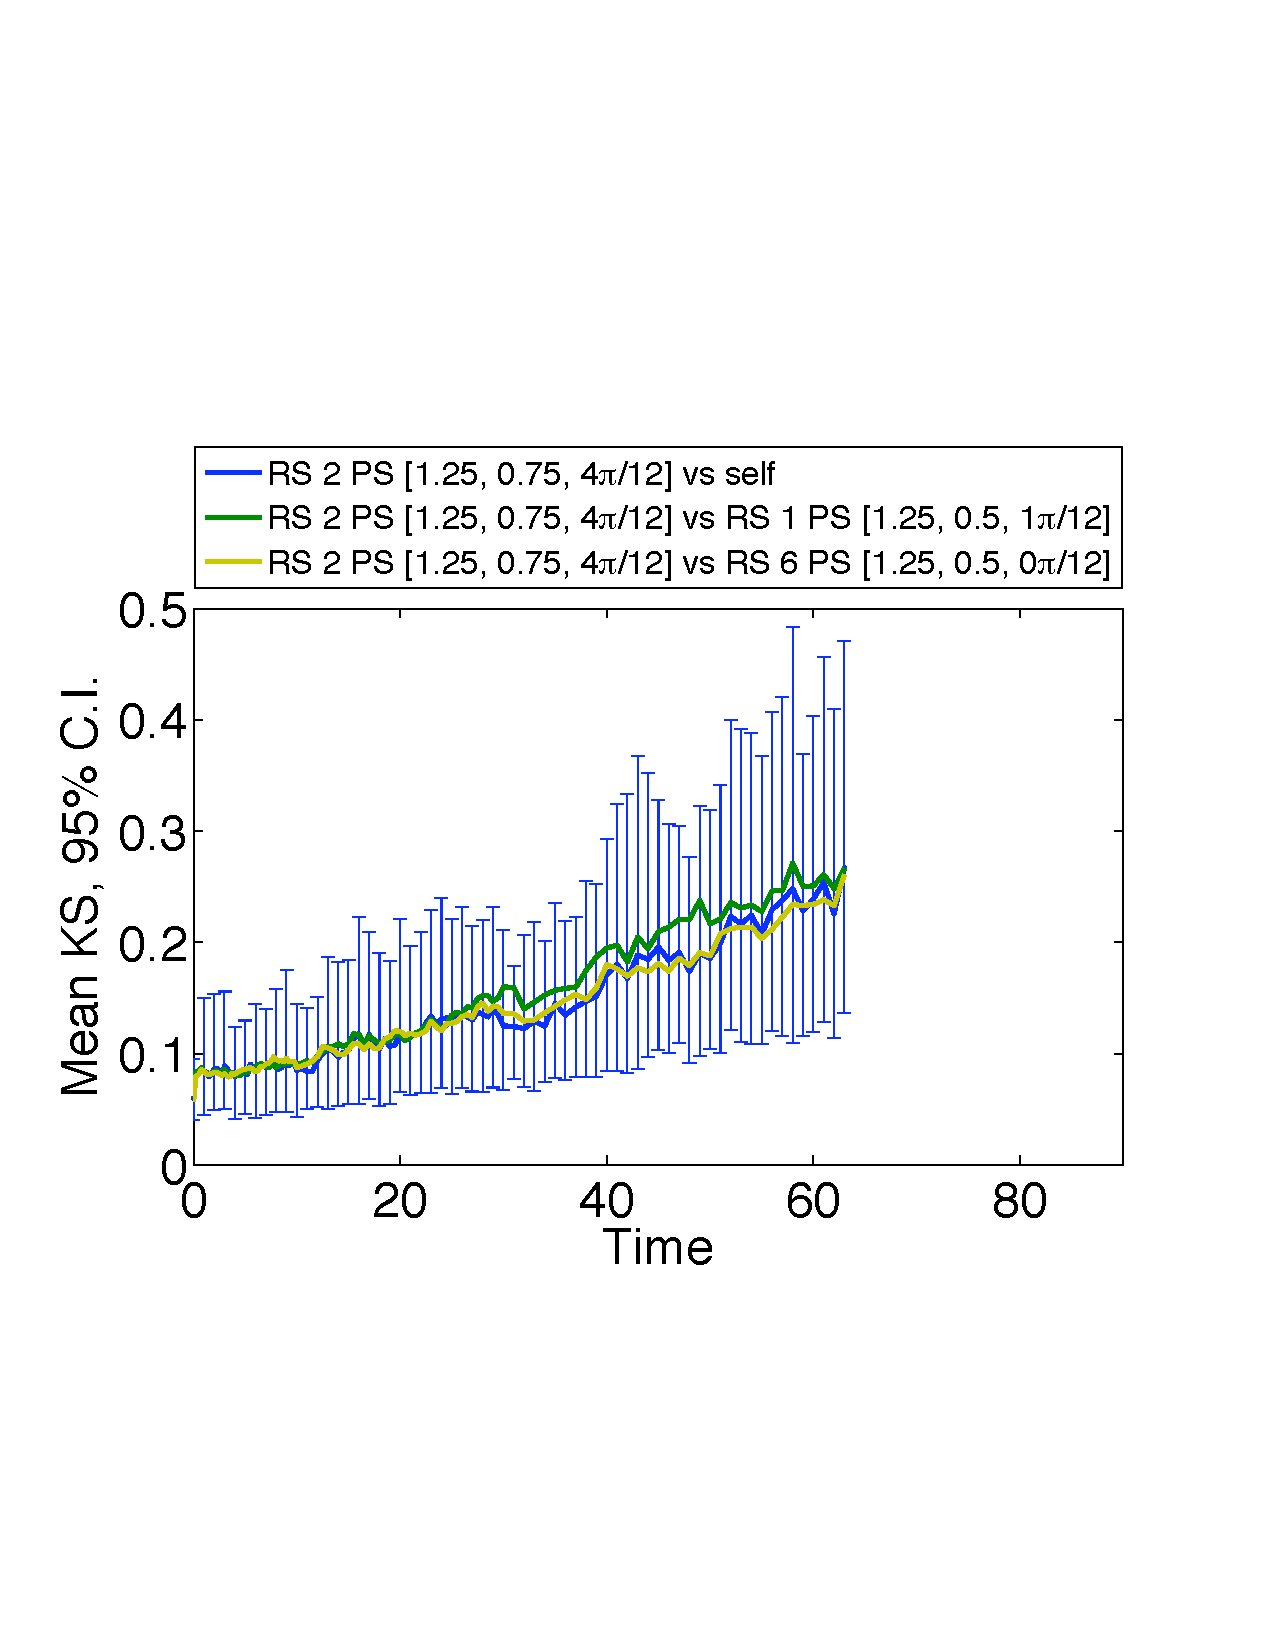
\includegraphics[width=3.25in]{figures/KSstatPerturb_RS02PS027_vs_RS01PS013_RS06PS012.pdf}} \\
% 	\multicolumn{2}{c}{A} \\
% 	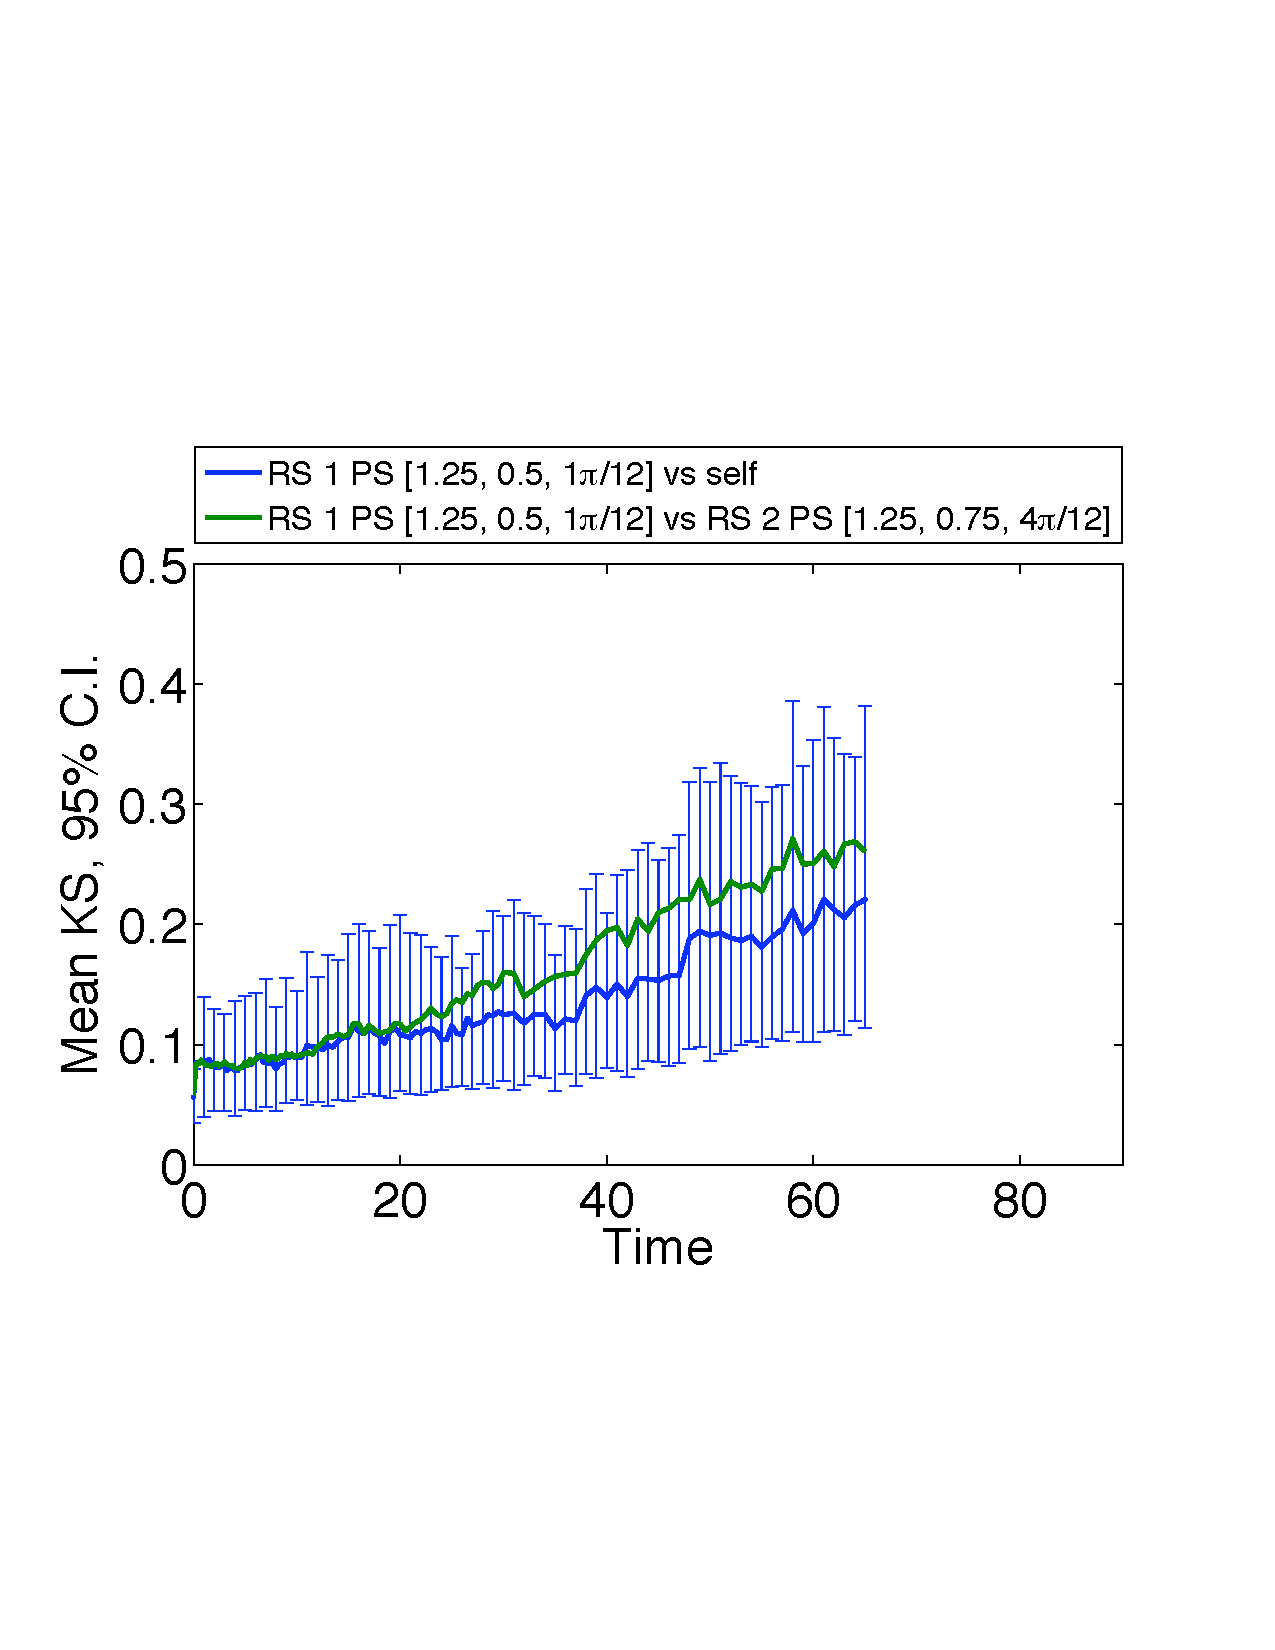
\includegraphics[width=3.25in]{figures/KSstatPerturb_RS01PS013_vs_RS02PS027.pdf} & 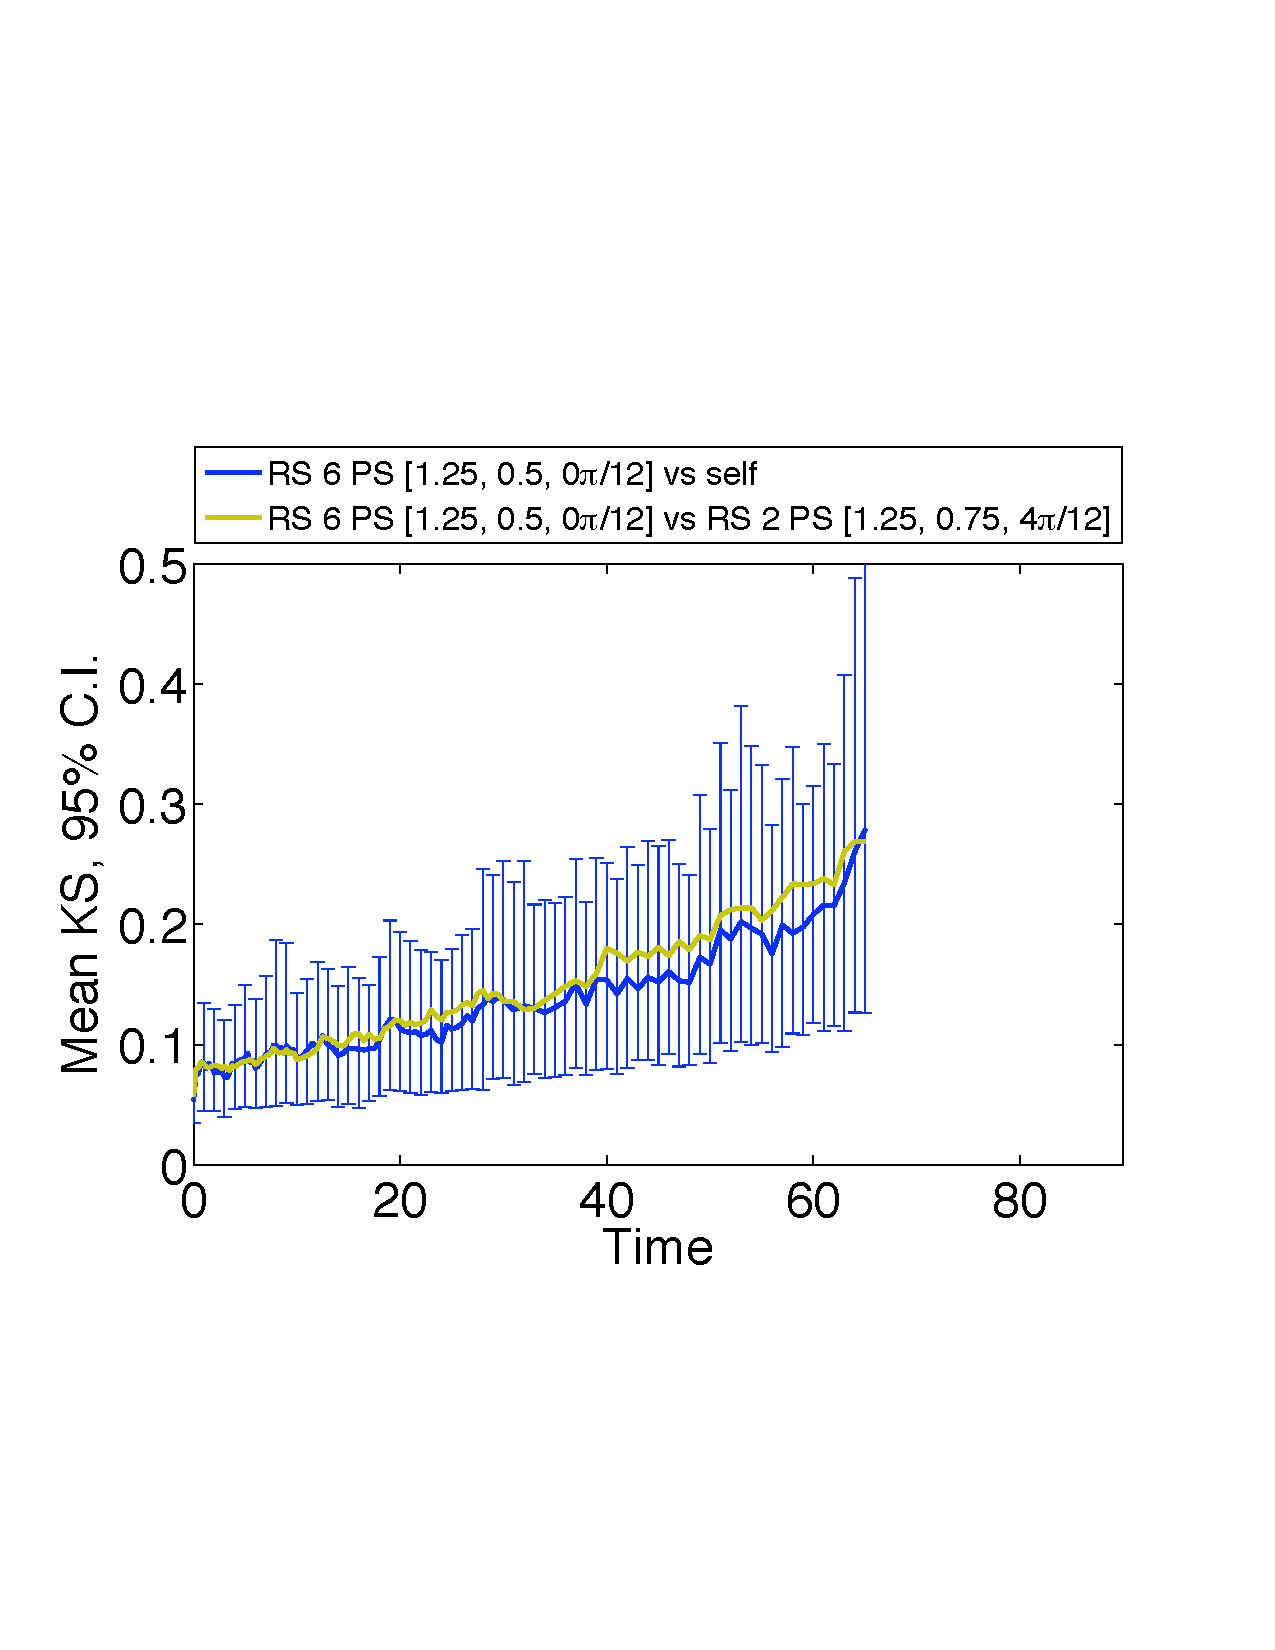
\includegraphics[width=3.25in]{figures/KSstatPerturb_RS06PS012_vs_RS02PS027.pdf}\\
% 	B & C \\
% \end{tabular}
% \caption{Rules 1 and 6 are still acceptable matches to rule 2 under perturbed conditions. Panel A uses the empirical distribution generated by rule 2 as the basis for comparison, while panels B and C use the distributions for rule 1 and rule 6 respectively. Notice that the relative goodness of the match depends on which empirical distribution is used for the comparison.}
% \label{ksperturb}
% \end{figure}
% 
% 
% 
% \section{Other comparisons with rule 2}\label{app:rule2matches}
% 
% Comparisons of rule 2 to rules 1, 6, and 10 (diffusion), may be seen in Figs.~\ref{fig:diffempdist}.B and \ref{fig:goodmatches}. Using the empirical distributions of rules 3-5 and 7-9, we exhibit the best matches to rule 2 that we could find below. All comparisons except to rules 3 and 4 show substantial dissimilarity. 
% 
% \begin{figure}[htp]
% \begin{tabular}{cc}
% 	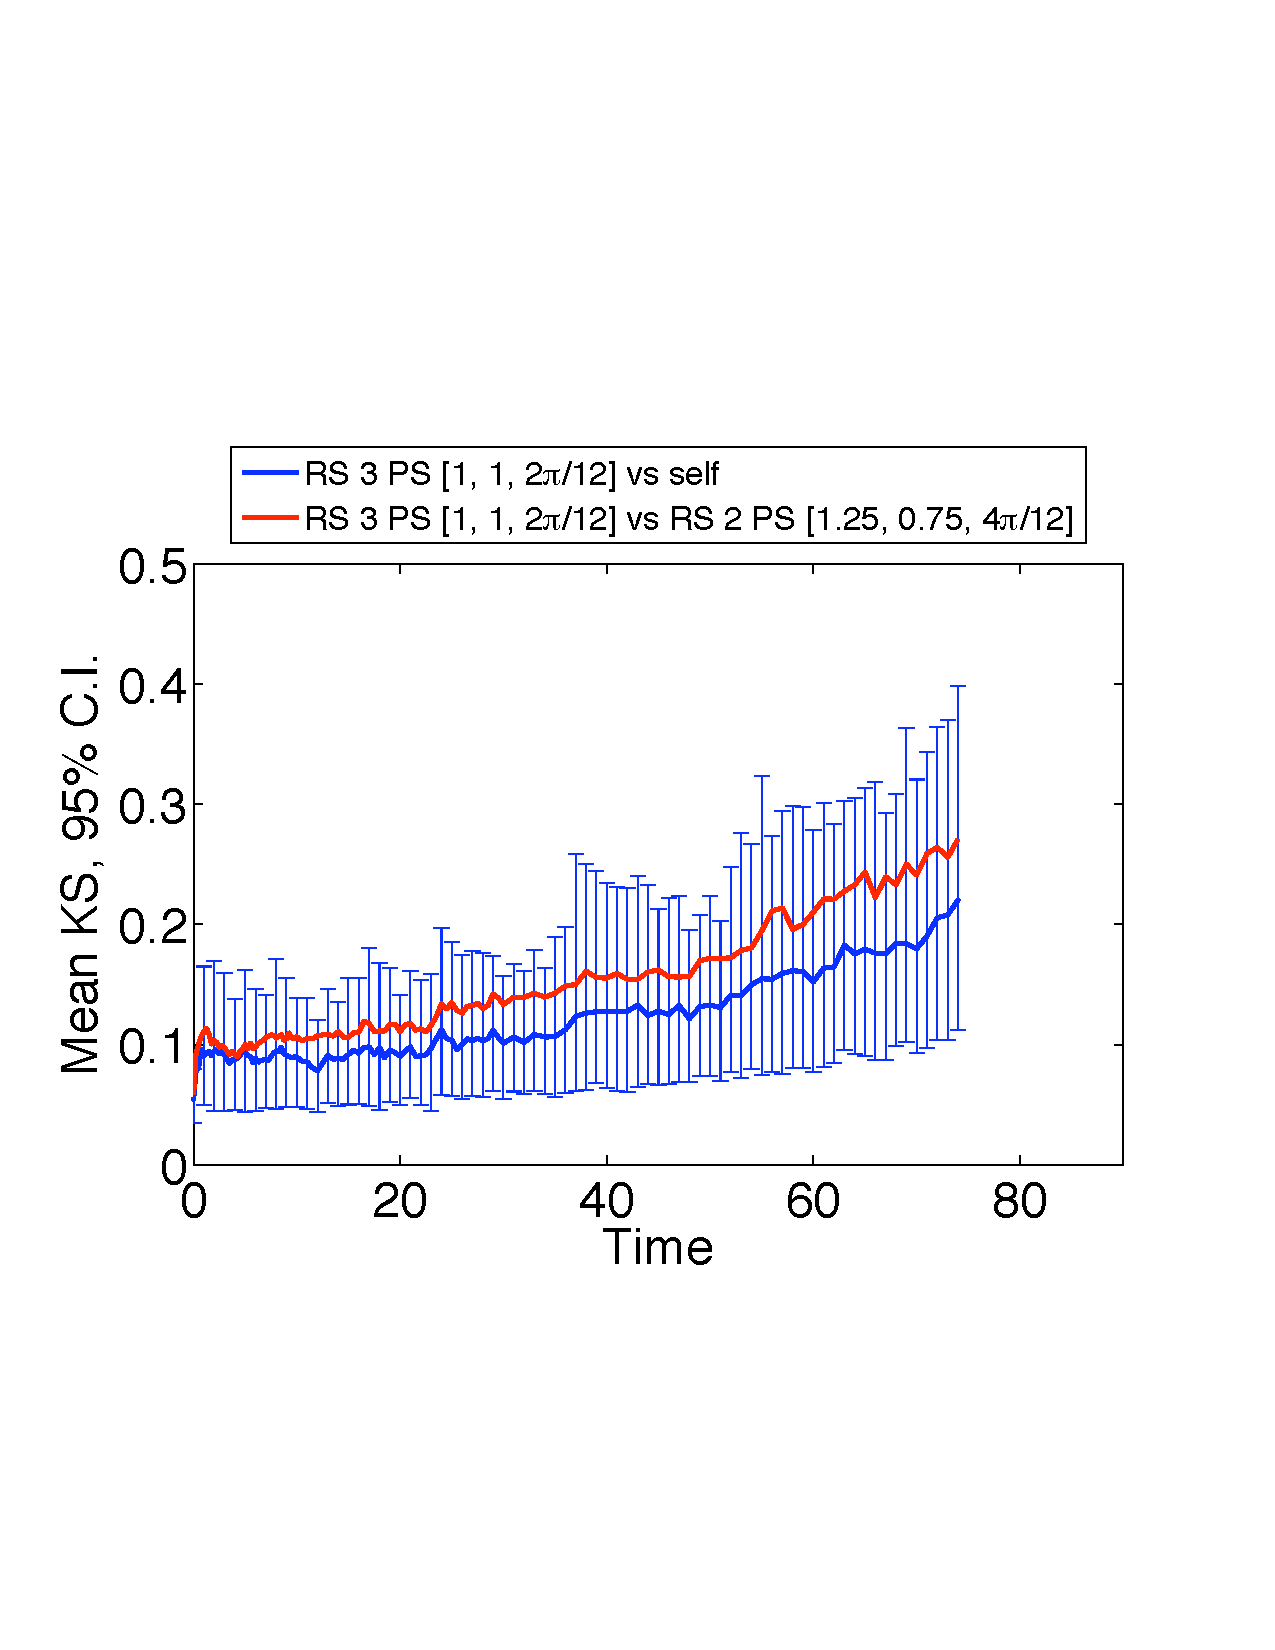
\includegraphics[width=3.25in]{KSstat_RS03PS091_vs_RS02PS027.pdf} & 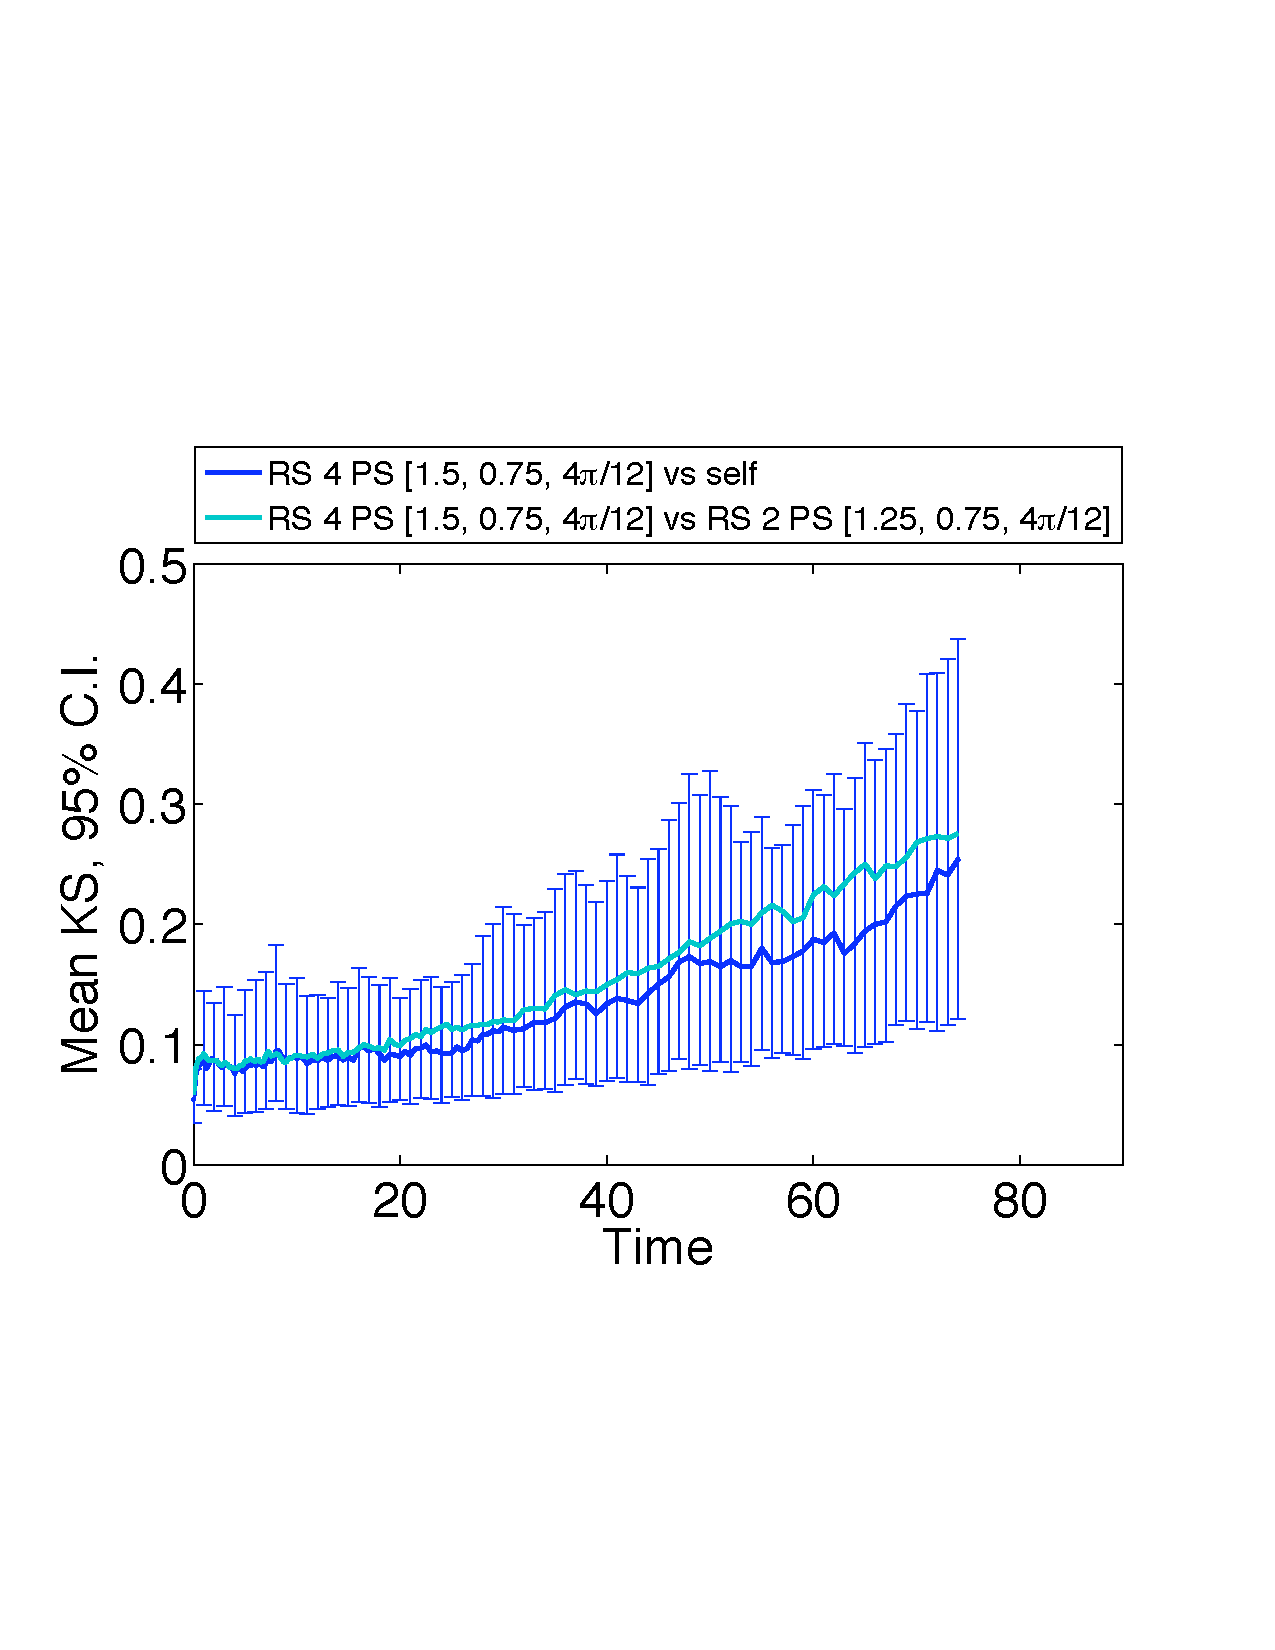
\includegraphics[width=3.25in]{KSstat_RS04PS060_vs_RS02PS027.pdf} \\
% 	A & B \\
% \end{tabular}
% \caption{Rules 3 and 4 are tolerable matches to rule 2.}
% \label{ksstatsopp3}
% \end{figure}
% 
% \begin{figure}[htp]
% \begin{tabular}{cc}
% 	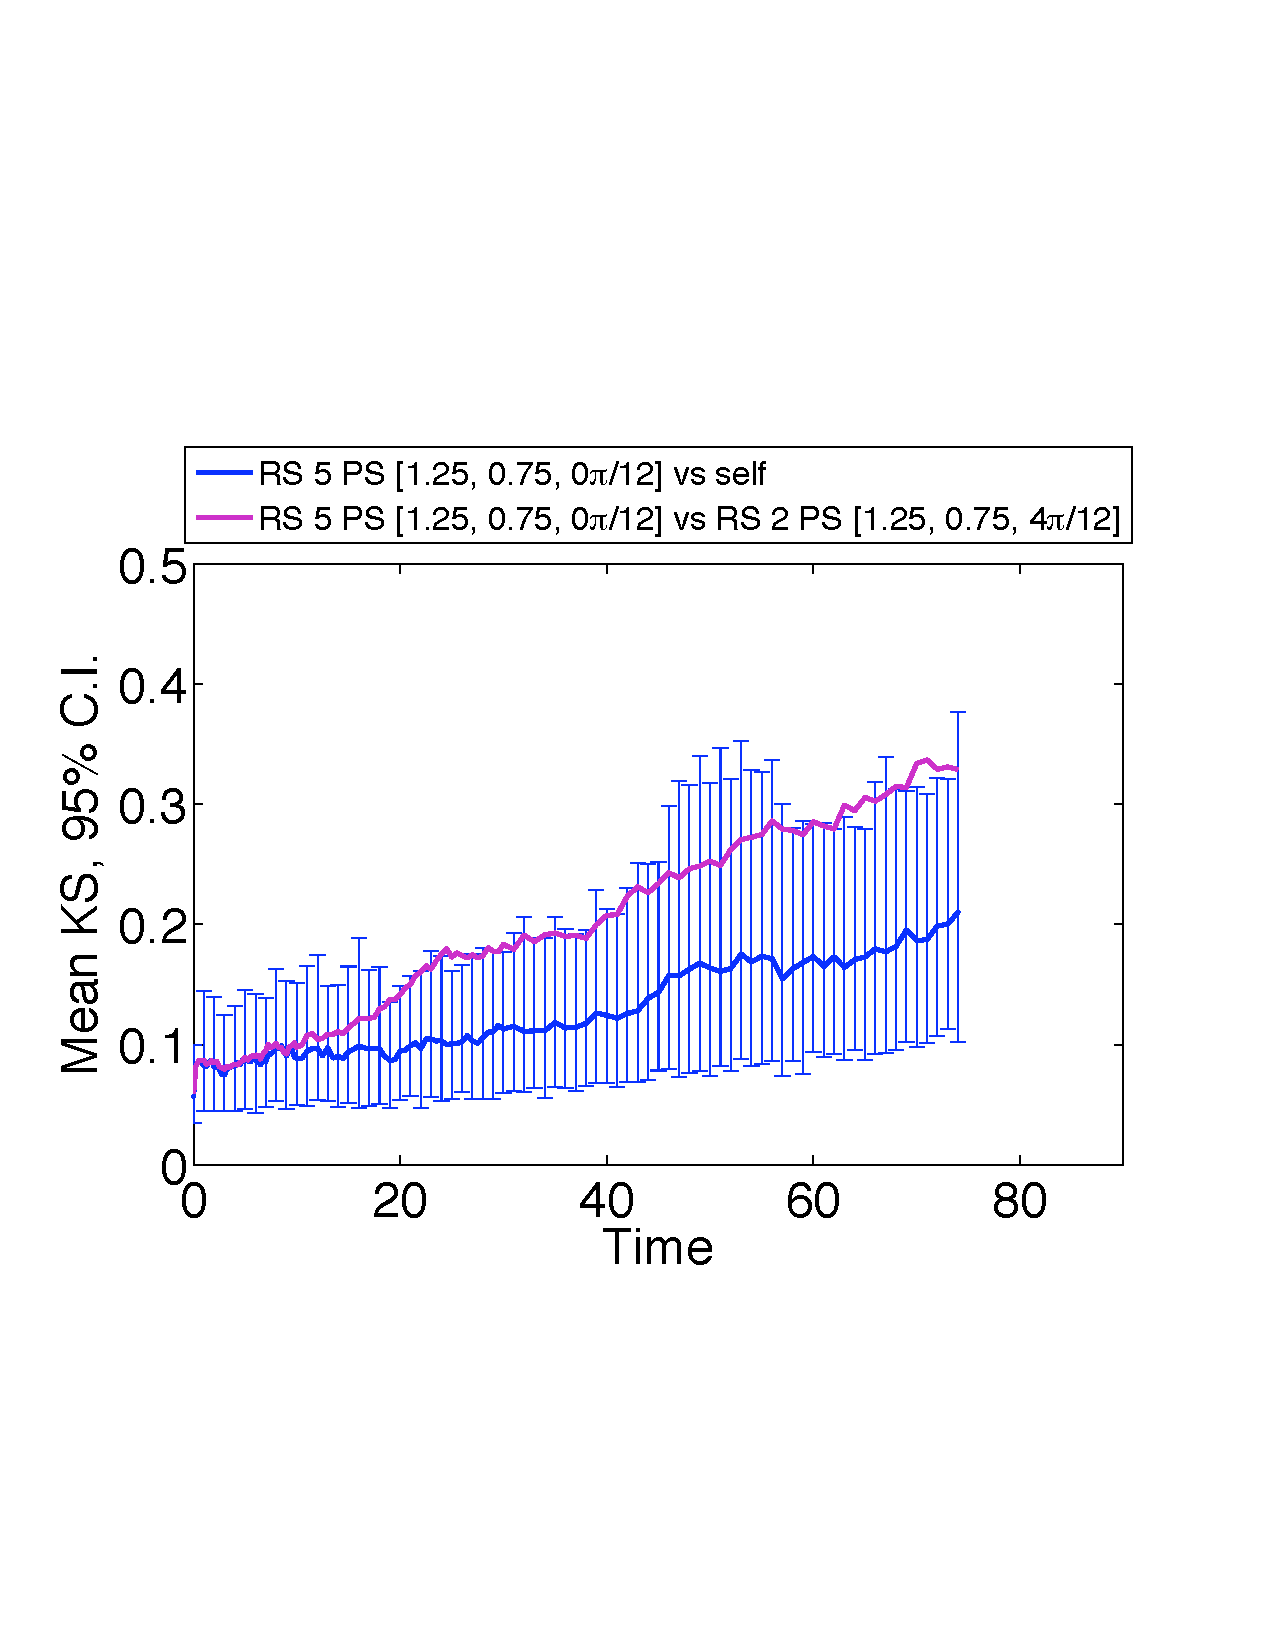
\includegraphics[width=3.25in]{KSstat_RS05PS023_vs_RS02PS027.pdf} & 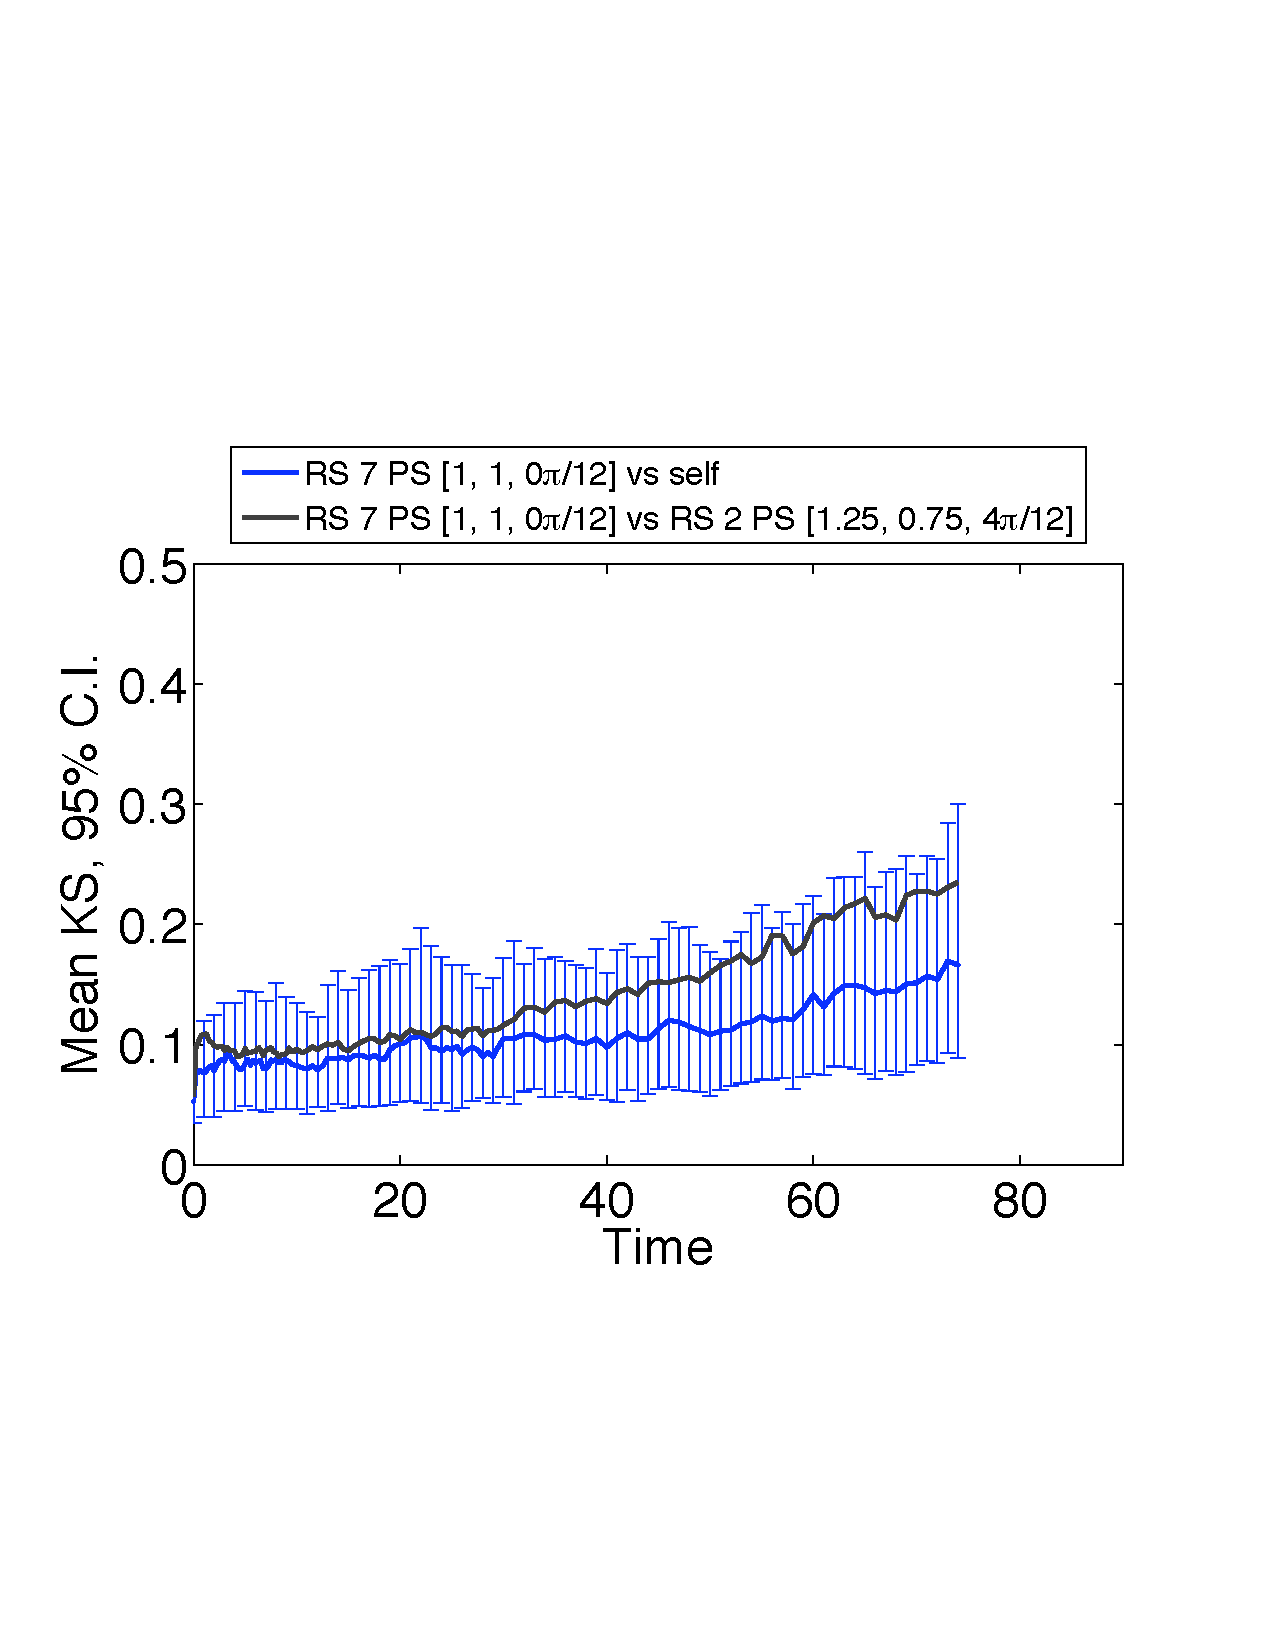
\includegraphics[width=3.25in]{KSstat_RS07PS023_vs_RS02PS027.pdf}\\
% 	A & B \\
% 	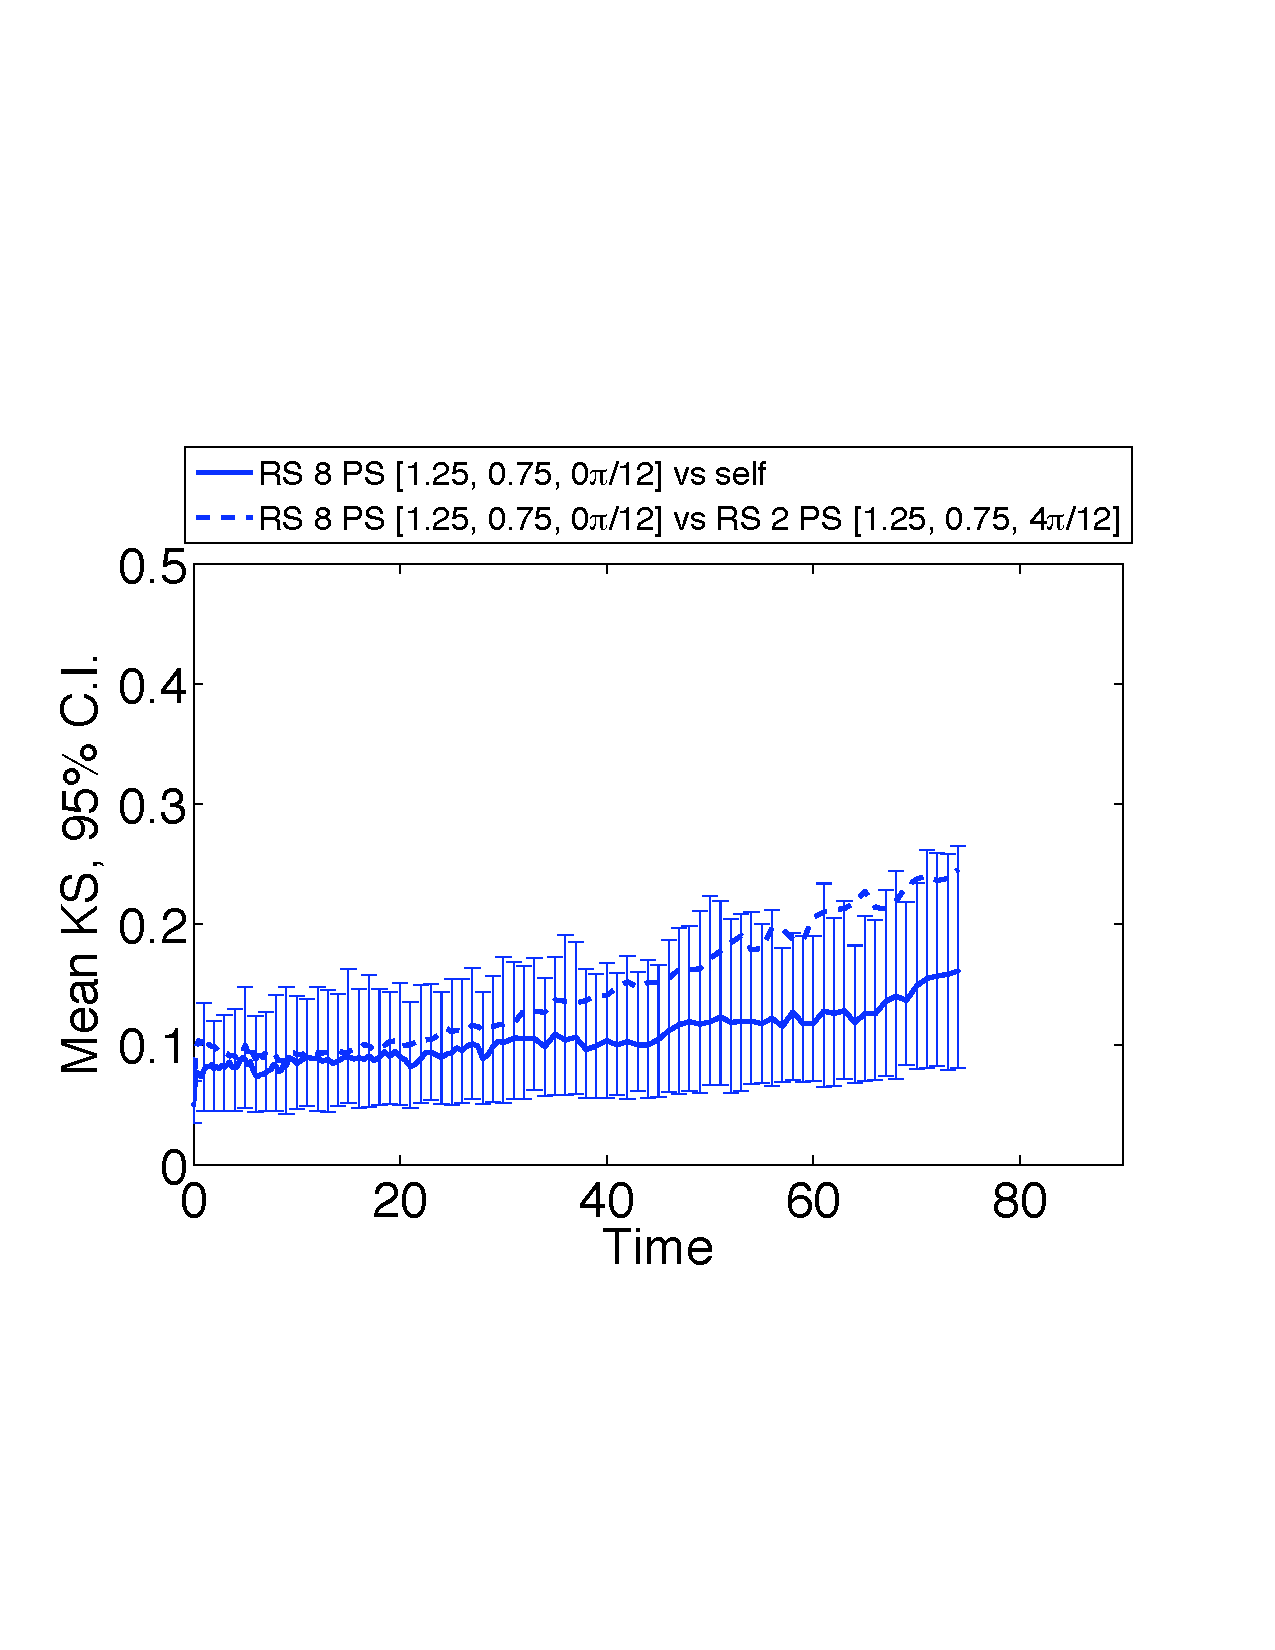
\includegraphics[width=3.25in]{KSstat_RS08PS023_vs_RS02PS027.pdf} & 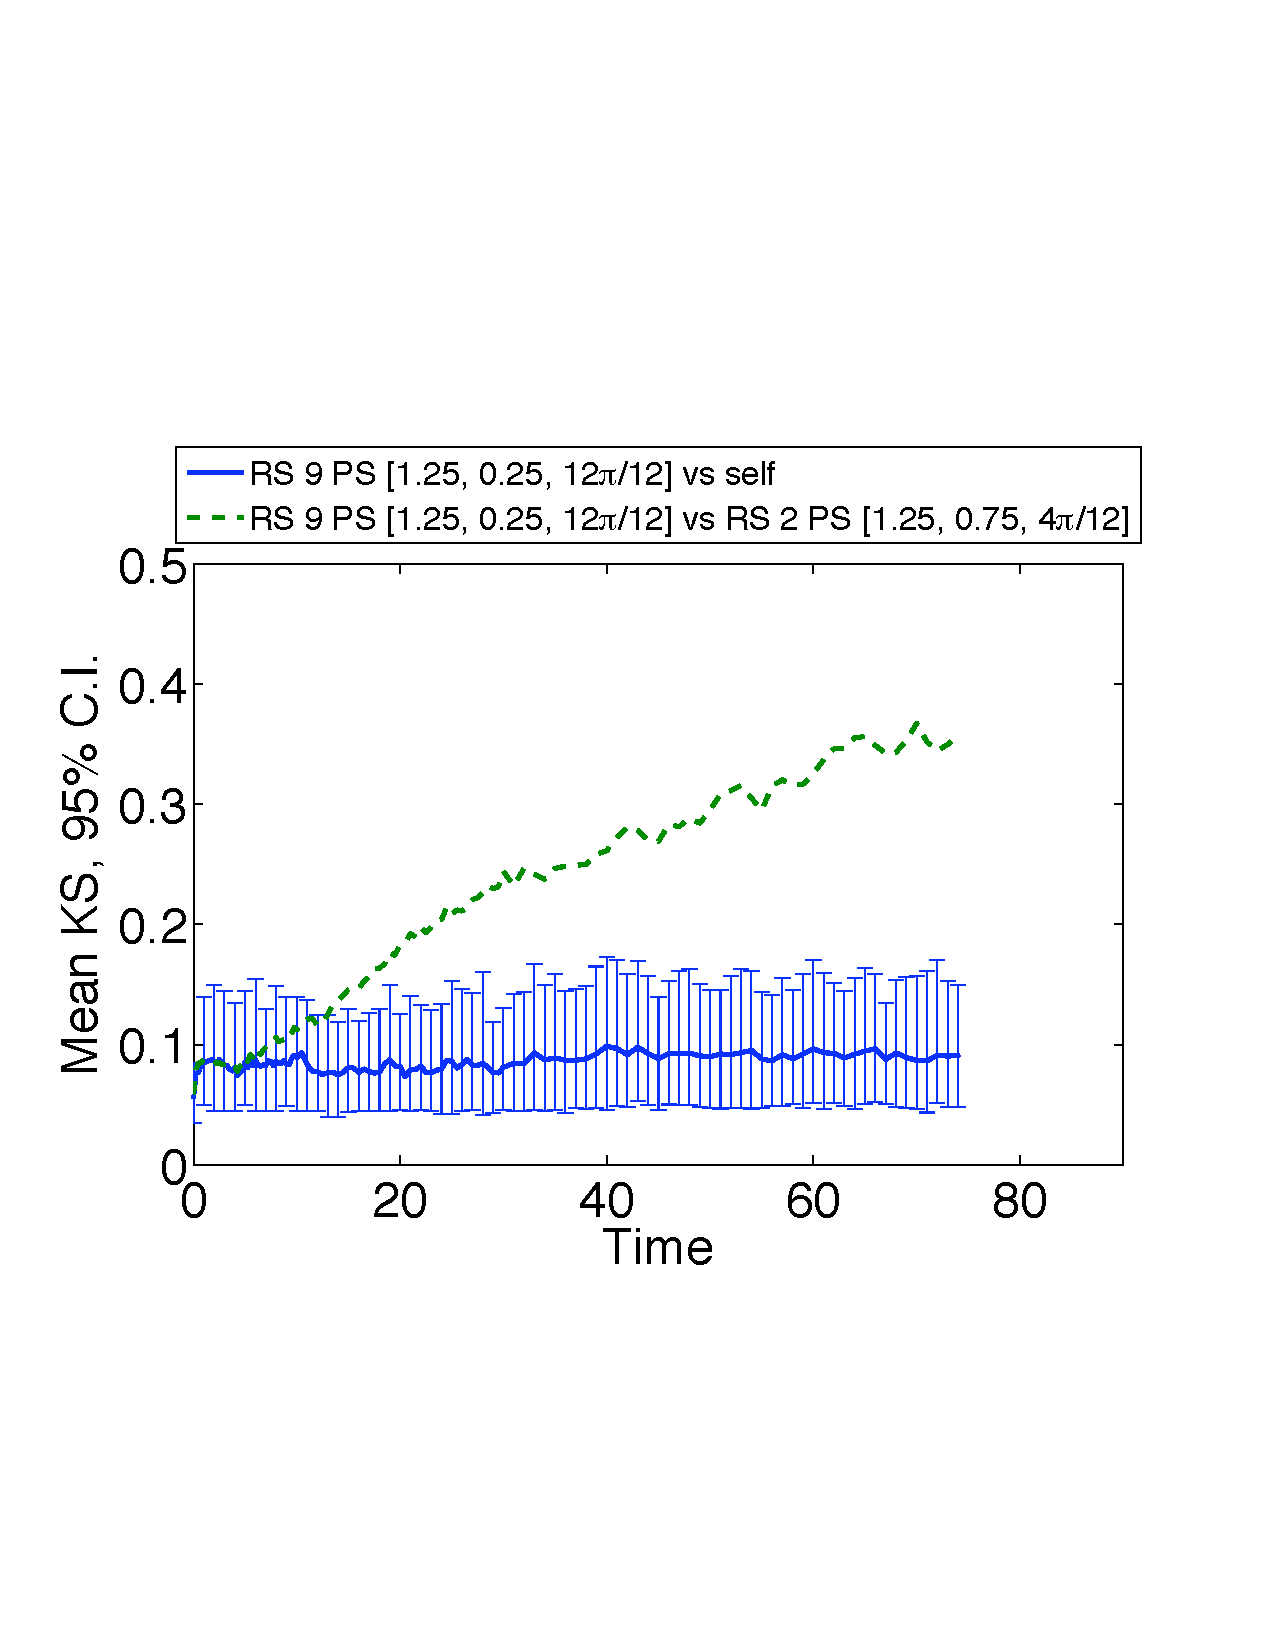
\includegraphics[width=3.25in]{KSstat_RS09PS008_vs_RS02PS027.pdf} \\
% 	C & D
% \end{tabular}
% \caption{Rules 5, 7, 8, and 9 are poor matches to rule 2.}
% \label{ksstatsopp2}
% \end{figure}
% 
% 
% \section{Sensitivity to response function concavity}\label{app:kappa}
% 
% The response function $F$ in Eq.~\ref{eqn:functional} depends on three parameters: a sensory threshold, $B_0$; a saturation level, $B_{sat}$; and a concavity parameter $\kappa$. We perform some minimal testing of the effect of these parameters on aggregate mosquito behavior using rule 2. In rule 2, we require thresholds and saturation levels for both CO$_2$ concentration ($C$) and for the CO$_2$ gradient ($G$). We fix the parameters $S_1 =  0.75$ m/s, $ S_2 = 1.25$ m/s, $ \beta_1 = \pi/3$, $C_0 = 0.027$ units CO$_2$ per unit air, and $G_0 = 4C_0/L$ units CO$_2$ per unit air per meter ($L$ is the length of one side of the domain). We let $C_{sat}$ vary between two values, 0.8 and 1, and the corresponding $G_{sat}$ is given by $4(C_{sat} - C_0) / L$. We also let $\kappa$ vary between three values, $\kappa_0 = 0$, $\kappa_1 = 200$, and the corresponding negative $\kappa_2$ which is the mirror reflection of $\kappa_1$: $\kappa_2 = -\kappa_1/(1 + \kappa_1 b_0 (1+b_0))$, where $b_0 = B_0/B_{sat}$. This means that there are two different $\kappa_2$, one for the concentration and one for the gradient. 
% 
% In total, there are six different parameter sets that we tested. Using the statistical methodology outlined in Section~\ref{sec:chemostats}, we compared all of them to the first parameter set ($\kappa = 0$ and $C_{sat} = 1$), which, except for $C_0 = 0$, is the parameter set for rule 2 that we have been exploring all along. We find only minor differences, and conclude that the model is not overly sensitive to the concavity of the response function (see Fig.~\ref{fig:kappa}). It seems likely to be equally insensitive to other classes of monotonic response functions, e.g. logistic functions. \comment{Bree: For completeness, I should look at the comparisons wrt the empirical distributions generated by the other rule sets. Empirical distributions 3 and 6 are farther from the others.}
% 
% \begin{figure}[htp]
% \begin{center}
% 	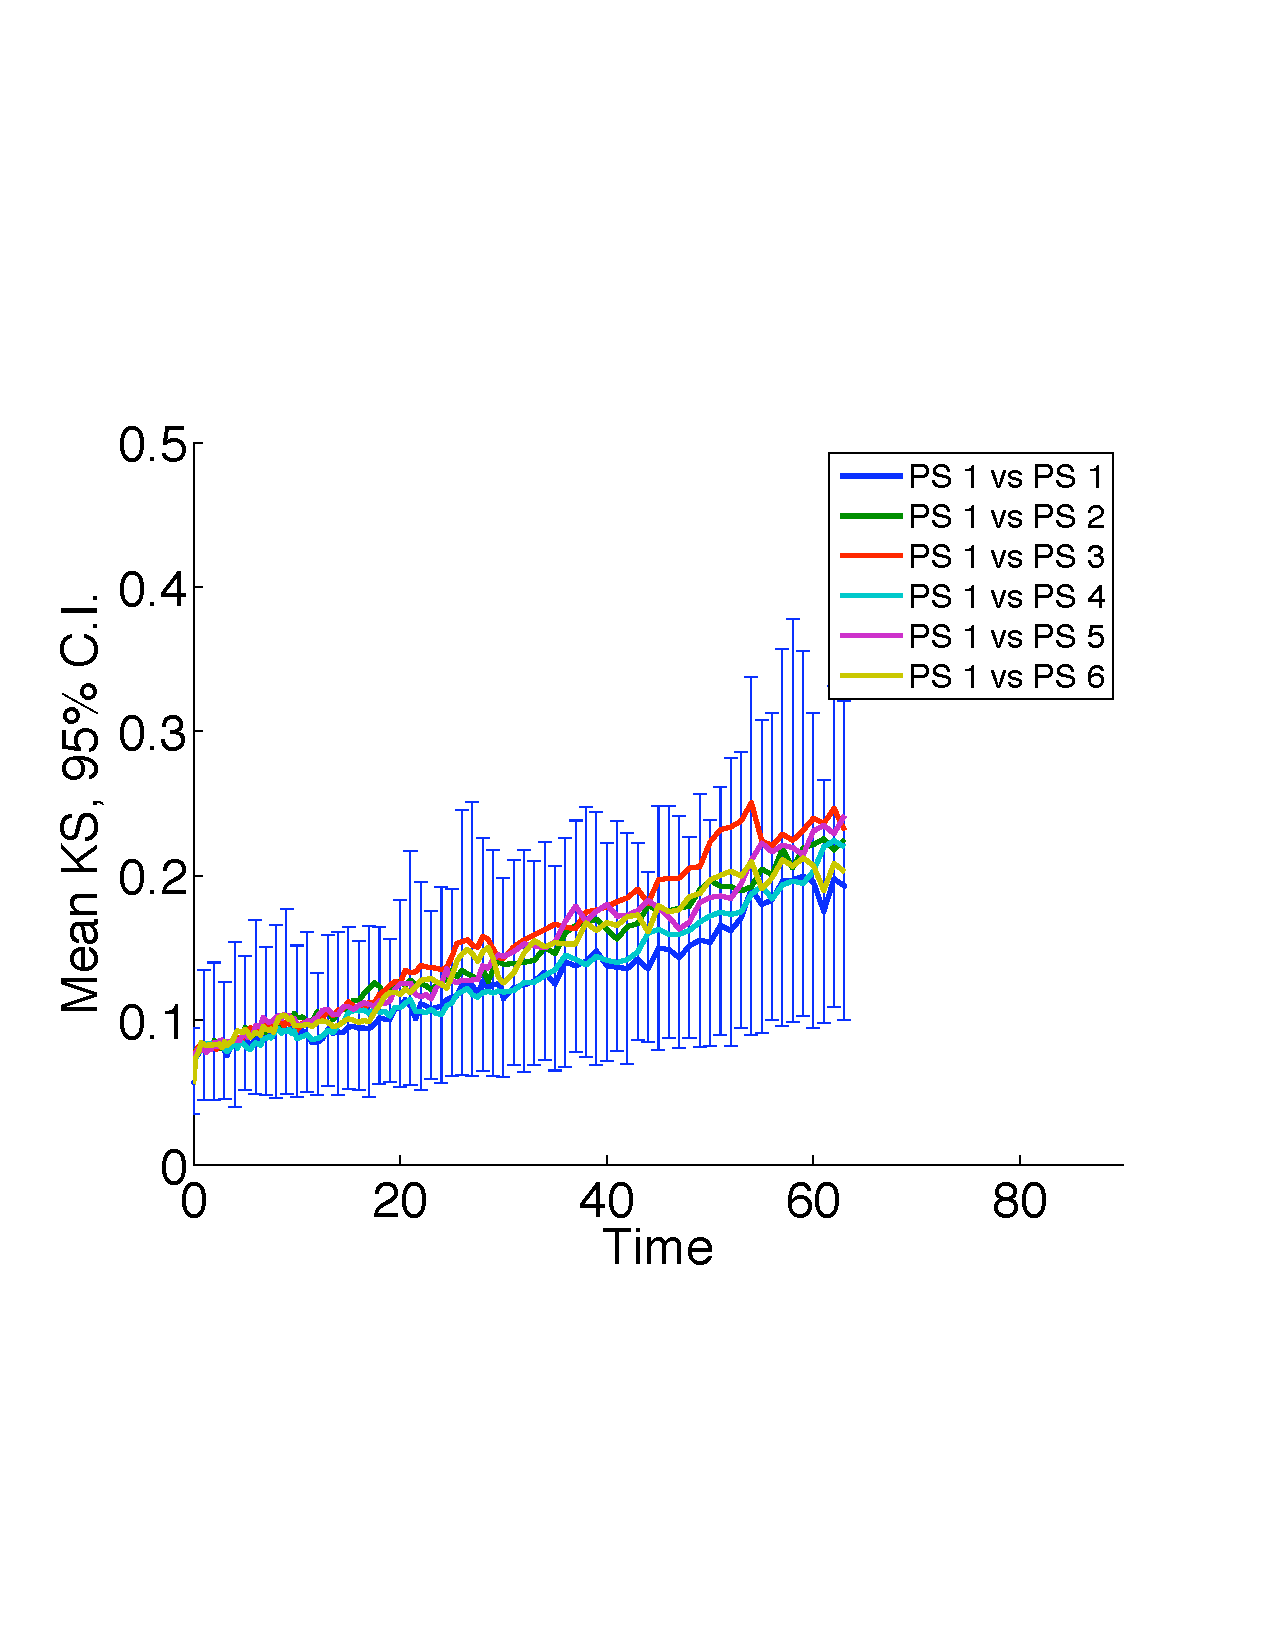
\includegraphics[width=4.0in]{kappacomparisons} 
% \end{center}
% \caption{Parameter sets (PS) 1 and 4 correspond to $\kappa_0$, 2 and 5 correspond to $\kappa_1$, and 3 and 6 correspond to $\kappa_2$. PS 1-3 have the higher saturation level. The linear functions ($\kappa_0$) are the most similar to each other, but all of the parameter sets are well within the confidence interval, indicating that in general they cannot be distinguished.}
% \label{fig:kappa}
% \end{figure}
\end{document}


